\documentclass[11pt]{article}

\usepackage[margin=1in]{geometry}
\usepackage{amsmath}
\usepackage{amssymb}
\usepackage{graphicx}
\usepackage{booktabs}
\usepackage{multirow}
\usepackage{xcolor}
\usepackage{float}
\usepackage{algorithm}
\usepackage{algpseudocode}
\usepackage{tikz}
\usetikzlibrary{arrows.meta,positioning,shapes.geometric}
\usepackage[numbers,sort&compress]{natbib}
\usepackage{hyperref}

\algnewcommand{\LineComment}[1]{\State \(\triangleright\) #1}
\algnewcommand{\Input}{\State \textbf{Input: }}
\algnewcommand{\Output}{\State \textbf{Output: }}

\hypersetup{
    colorlinks=true,
    linkcolor=blue,
    citecolor=blue,
    urlcolor=blue
}

\title{From Accurate Forecasts to Feasible Plans: Feasibility-Constrained Model Selection for Operational Demand Planning}
\author{Author Name Placeholder}
\date{\today}

\begin{document}

\maketitle

\begin{abstract}
Forecasting models for operational demand planning are often evaluated by numerical prediction accuracy, yet operational systems do not execute forecasts directly. They execute planning signals such as inventory targets, replenishment recommendations, staffing plans, or capacity allocations. A forecast that improves error metrics can still produce volatile or infeasible plans when downstream execution capacity, model-switching burden, inventory exposure, and planning stability are ignored. This paper formulates forecast-driven demand planning as a feasibility-constrained model selection problem. The proposed evaluation layer converts candidate forecasts into executable planning signals and compares deployable strategies using both raw operational metrics and a normalized planning utility that includes inventory cost, planning volatility, switching burden, and execution violations. Empirically, this study uses DataCo supply-chain execution data to anchor execution-risk scenarios, Favorita retail demand data as the main forecast-to-plan proof of concept, M5 retail demand data as a hierarchical robustness setting, and Walmart data as a weekly business-context robustness check. Across the current paper-facing evaluations, the accuracy-first deployable method is not the operational-loss-optimal deployable strategy in 91.1\% of 123 evaluation groups. The current results suggest that execution-risk-sensitive objectives can reorder deployable strategy rankings, without implying that any single strategy universally dominates. The implication is that operational feasibility should be treated as a first-class planning objective alongside forecast accuracy.

\end{abstract}

\section{Introduction}

Demand planning increasingly relies on predictive models to anticipate future demand at fine operational granularity. In many empirical studies and model-selection workflows, the primary criterion for choosing among forecasting methods is numerical prediction accuracy. Metrics such as mean absolute error, root mean squared error, and weighted absolute percentage error are important because inaccurate forecasts can lead to costly overstocking, stockouts, and service failures. However, forecast accuracy alone does not describe whether the resulting plan can be executed.

In real operations, forecasts are not executed directly. A forecast is converted into a planning signal: an inventory target, a replenishment quantity, a labor plan, a production target, a transportation commitment, or an allocation decision. This forecast-to-plan conversion is mediated by business policies, service-level targets, safety-stock rules, system constraints, and planner review processes. The operational question is therefore not only whether a forecast is numerically close to realized demand, but whether the planning signal implied by that forecast is stable, feasible, and worth deploying.

A more accurate forecast may create unstable planning signals. It may require frequent model switching, large period-to-period target jumps, repeated infrastructure updates, or adjustment requests that exceed what suppliers, stores, warehouses, transportation teams, and enterprise planning systems can absorb. These burdens may be invisible in forecast-error tables. A model that looks attractive under WAPE can still be unattractive when it generates plan churn, execution violations, or additional governance work.

This creates a planning-execution gap. Forecasting capability can adapt faster than downstream execution infrastructure. Machine learning pipelines may update daily or weekly, while procurement lead times, labor scheduling, supplier coordination, production planning, and information-system workflows may change more slowly. When the forecasting layer changes faster than the execution layer can absorb, prediction accuracy and deployable planning quality can diverge.

This paper studies forecast-driven demand planning as a feasibility-constrained model selection problem. Rather than asking which forecasting model has the lowest error in isolation, the paper asks which deployable planning strategy balances forecast accuracy, inventory exposure, planning volatility, model-switching burden, and execution-capacity constraints. The objective is not to argue that stability-aware or feasibility-aware strategies always dominate. The objective is to make the tradeoff surface visible and to evaluate model selection in the same operational space where planning decisions are executed.

The empirical design uses three public-data roles. DataCo supply-chain execution data is used to show that execution risk is empirically measurable and to construct data-informed execution-risk sensitivity scenarios. Favorita retail demand data provides the main forecast-to-plan proof of concept, with demand, promotion, holiday, oil-price, transaction, and store-context signals. M5 provides a larger hierarchical retail robustness setting across item, department, category, store, and state levels. Walmart and Rossmann are reserved as optional future robustness extensions; no results from those datasets are claimed in the current draft.

The paper makes four contributions. First, it formulates forecast-driven demand planning as feasibility-constrained model selection, separating forecast generation from the downstream choice of a deployable planning strategy. Second, it defines a normalized planning utility that compares inventory exposure, planning volatility, switching burden, and execution violations relative to an accuracy-first baseline while still reporting raw operational metrics. Third, it constructs DataCo-informed execution-risk scenarios as sensitivity anchors, without claiming exact economic cost calibration between DataCo and the demand-planning datasets. Fourth, it shows empirically that execution-risk-sensitive objectives can reorder deployable strategy rankings and that the preferred deployable method depends on execution scenario, planning granularity, and demand intermittency.

\section{Related Work}

\subsection{Demand Forecasting and Inventory Implications}

Demand forecasting research studies how predictive models can estimate future demand across products, stores, regions, and time periods. A closely related stream connects forecast quality to downstream inventory and service outcomes. This paper builds on that operational motivation but focuses on an intermediate layer that is often left implicit: the conversion of candidate forecasts into planning signals that must be executed under finite adjustment capacity.

% TODO: cite demand forecasting and inventory-control literature.

\subsection{Forecast Combination and Model Selection}

Forecast-combination and model-selection methods provide mechanisms for choosing among or aggregating candidate forecasts. Standard selection criteria often prioritize forecast error on validation data. The present paper differs by evaluating deployable planning utility rather than forecast error alone. A forecast combination can be attractive not only because it improves accuracy, but because it reduces abrupt plan changes, spreads model risk, or avoids unnecessary switching.

% TODO: cite forecast combination and model-selection literature.

\subsection{Cost-Sensitive and Multi-Objective Decision Making}

Cost-sensitive and multi-objective decision methods are related because demand planning rarely has a single objective. Inventory cost, service level, volatility, and execution burden can move in different directions. The contribution here is not a generic multi-objective optimizer. It is a structured operational planning evaluation framework in which forecast-driven plans are compared against execution-capacity constraints and normalized relative to an accuracy-first baseline.

% TODO: cite cost-sensitive learning and multi-objective optimization literature.

\subsection{Supply-Chain Execution Risk and Planning Stability}

Supply-chain execution risk, planning nervousness, and plan volatility are central to the gap studied in this paper. Downstream operations may be unable to absorb large changes in inventory targets, replenishment quantities, transportation commitments, or staffing plans. This paper connects forecast-driven model selection to measurable execution feasibility by using supply-chain execution evidence to define scenario weights and by evaluating planning volatility and execution violations directly.

% TODO: cite supply-chain execution risk, planning nervousness, and volatility literature.

\section{Problem Formulation}

\subsection{Planning Units and Candidate Forecasts}

Let $i$ index a planning unit, such as an item-store or store-family pair, and let $t$ index a planning period. Let $m \in \mathcal{M}$ denote a candidate forecasting model. Actual demand is denoted by $y_{i,t}$, and the forecast produced by model $m$ is denoted by $\hat{y}_{i,t}^{m}$.

The forecasting layer produces a set of candidate forecasts:
\begin{equation}
    \left\{\hat{y}_{i,t}^{m}: m \in \mathcal{M}\right\}.
\end{equation}

The decision layer converts these candidate forecasts into a final forecast signal $\tilde{y}_{i,t}$ and then into an executable planning signal $x_{i,t}$.

\subsection{Hard Model Selection}

Under hard model selection, the decision layer selects one model $z_{i,t} \in \mathcal{M}$ for each planning unit and period:
\begin{equation}
    \tilde{y}_{i,t} = \hat{y}_{i,t}^{z_{i,t}}.
\end{equation}

Hard selection is operationally meaningful because changing $z_{i,t}$ can require model validation, monitoring changes, deployment updates, and planner communication.

\subsection{Soft Model Composition}

Under soft model composition, the decision layer assigns a nonnegative weight $w_{i,t}^{m}$ to each candidate model:
\begin{equation}
    \tilde{y}_{i,t} = \sum_{m \in \mathcal{M}} w_{i,t}^{m}\hat{y}_{i,t}^{m}.
\end{equation}

The weights satisfy:
\begin{align}
    w_{i,t}^{m} &\geq 0, \\
    \sum_{m \in \mathcal{M}} w_{i,t}^{m} &= 1.
\end{align}

Soft composition can reduce hard model switching, but large weight changes may still create governance and monitoring burden.

\subsection{Planning Signal Conversion}

The operation executes a planning signal rather than a raw forecast. In this initial formulation, the planning signal is an inventory target:
\begin{equation}
    x_{i,t} = \tilde{y}_{i,t} + \text{safety\_stock}_{i,t}.
\end{equation}

The same framework can later represent other executable signals, including replenishment quantities, production targets, staffing levels, or capacity allocations.

\subsection{Inventory Cost}

Inventory cost includes holding cost for over-planning and shortage cost for under-planning:
\begin{align}
    \text{holding\_cost}_{i,t} &= h \max(x_{i,t} - y_{i,t}, 0), \\
    \text{shortage\_cost}_{i,t} &= p \max(y_{i,t} - x_{i,t}, 0), \\
    \text{inventory\_cost}_{i,t} &= \text{holding\_cost}_{i,t} + \text{shortage\_cost}_{i,t},
\end{align}
where $h$ is the holding cost rate and $p$ is the shortage cost rate.

\subsection{Planning Signal Volatility}

Planning signal volatility measures how sharply the executable signal changes across periods:
\begin{equation}
    \text{plan\_change\_pct}_{i,t}
    =
    \frac{|x_{i,t} - x_{i,t-1}|}{\max(|x_{i,t-1}|, \epsilon)}.
\end{equation}

This term captures plan churn that may be invisible in forecast error metrics.

\subsection{Model Switching Cost}

For hard selection, model switching cost is:
\begin{equation}
    \text{switch\_cost}_{i,t}
    =
    \begin{cases}
    1, & z_{i,t} \neq z_{i,t-1}, \\
    0, & z_{i,t} = z_{i,t-1}.
    \end{cases}
\end{equation}

For soft composition, the analogous instability measure is total weight movement:
\begin{equation}
    \text{weight\_change}_{i,t}
    =
    \sum_{m \in \mathcal{M}}
    |w_{i,t}^{m} - w_{i,t-1}^{m}|.
\end{equation}

\subsection{Execution Adaptation Penalty}

Let $C_{i,t}$ denote execution capacity, defined as the maximum plan change the operation can absorb in period $t$. The execution adaptation penalty is:
\begin{equation}
    \text{execution\_penalty}_{i,t}
    =
    \max\left(0, |x_{i,t} - x_{i,t-1}| - C_{i,t}\right).
\end{equation}

This penalty captures the planning-infrastructure gap. It becomes positive when the forecast or planning signal changes faster than execution infrastructure can absorb. In practical terms, the forecasting layer may update rapidly, while procurement, staffing, production, transportation, software systems, or planner workflows may only absorb smaller or slower changes.

\subsection{Multi-objective Planning Loss}

The project evaluates planning utility through a multi-objective loss:
\begin{align}
    \text{total\_loss}
    ={}&
    \alpha \cdot \text{forecast\_error}
    + \beta \cdot \text{inventory\_cost} \notag \\
    &+ \lambda_{\text{volatility}} \cdot \text{planning\_signal\_volatility} \notag \\
    &+ \lambda_{\text{switch}} \cdot \text{model\_switching\_cost} \notag \\
    &+ \lambda_{\text{execution}} \cdot \text{execution\_adaptation\_penalty}.
\end{align}

The weighted scalar loss is useful for optimization and policy comparison. The paper will also report Pareto-style multi-objective outputs so that tradeoffs among accuracy, inventory cost, stability, switching, and execution adaptation remain visible.

\section{Framework and Methods}

\subsection{Framework Overview}

The framework separates forecast generation from deployable planning strategy selection. Candidate forecasting models first produce forecasts for each planning unit and period. A decision layer then selects, combines, or smooths the candidate signals before converting them into executable planning signals. The resulting plans are evaluated using both forecasting metrics and operational metrics that reflect inventory exposure, plan volatility, model-switching burden, and execution-capacity violations.

This structure is designed to evaluate deployable strategy families rather than only individual forecasting models. A method can be attractive because it is accurate, because it produces stable plans, because it reduces execution burden, or because it offers a favorable balance among these objectives. The empirical design therefore reports raw metrics and normalized planning loss rather than reducing the analysis to a single forecasting leaderboard.

\subsection{Accuracy-First Methods}

Accuracy-first methods select forecasts using validation or test-period forecast accuracy. The Global Best or BestAccuracy strategy applies the numerically strongest candidate model globally. The Family Best strategy allows model choice to vary by product family or comparable planning group. These strategies are important baselines because they represent the common deployment logic of choosing the best forecaster before considering downstream execution consequences.

\subsection{Stability-First Methods}

Stability-first methods prioritize low plan volatility. In the current experiments, moving-average and BestStability variants serve as deliberately conservative references. They are not included to claim that simple smoothing is always better than machine learning. They are included because an over-stable but weak baseline helps identify the operational cost of suppressing plan changes too aggressively.

\subsection{Ensemble-Based Methods}

The Simple Ensemble averages candidate forecasts without using operational-loss information. It provides a transparent reference for forecast combination. The Operational-Loss Ensemble assigns nonnegative weights that sum to one using validation normalized planning loss rather than forecast error alone. This family tests whether soft forecast composition can preserve useful accuracy while reducing abrupt execution burden.

\subsection{Smoothing-Based Methods}

FeasibilityAwareSmoothed strategies modify the executed planning signal after a candidate plan is formed. With fixed-alpha smoothing, the adaptation rate is configured directly. With utility-CV smoothing, the adaptation rate is selected from a small validation grid using blocked validation folds to reduce dependence on a single validation period. The smoothing equation is
\begin{equation}
    x_{i,t}^{\mathrm{exec}}
    =
    \alpha_{t} x_{i,t}^{\mathrm{cand}}
    +
    (1-\alpha_{t})x_{i,t-1}^{\mathrm{exec}}.
\end{equation}
Smoothing changes the executed planning signal, not the underlying demand realization and not the raw forecast itself. It is intended to model gradual operational adaptation when execution infrastructure cannot absorb abrupt target changes.

\subsection{Feasibility-Aware Adaptive Selection}

The Feasibility-Aware Selector evaluates candidate model changes using expected planning utility rather than forecast error alone. In the default operational objective, it considers expected inventory cost, planning volatility, model-switching burden, and expected execution violations; forecast error remains a reported diagnostic unless an explicit sensitivity setting assigns it positive weight. A switch is accepted only when the expected planning utility improves after feasibility penalties. This method is intentionally interpretable; it is not a reinforcement-learning or black-box control policy.

\subsection{Finite-Horizon DP Selection}

The GreedyFeasibilitySelector minimizes the current-period expected operational cost using validation-derived model costs and current forecast-implied transition costs. It is a one-step policy and can switch when the immediate score improves.

The DPFeasibilitySelector solves the deterministic finite-horizon model-selection problem for each planning series. Its state is the previously selected model, which determines the previous planning signal and therefore the next transition cost. The DP minimizes cumulative expected operational loss over the available horizon using validation-derived expected costs; it does not use realized test demand.

The finite-horizon DP is used to quantify the value of planning ahead under switching and execution costs. Greedy selection is a one-step policy, while DP minimizes cumulative loss over the horizon. The greedy-to-DP gap therefore measures myopic selection suboptimality under the same validation-derived cost information.

\begin{center}
\fbox{\begin{minipage}{0.92\linewidth}
\textbf{Proposition 1 (Greedy selection as one-step DP).}
Let $c_t(m \mid m_{t-1}, x_{t-1})$ denote the validation-derived stage cost of choosing model $m$ at period $t$, conditional on the previous model $m_{t-1}$ and previous executed planning signal $x_{t-1}$. The finite-horizon DP value function is
\begin{equation}
V_t(m_{t-1}, x_{t-1})
=
\min_{m \in \mathcal{M}_t}
\left\{
c_t(m \mid m_{t-1}, x_{t-1})
+ V_{t+1}(m, x_t^{m})
\right\},
\quad
V_{T+1}=0.
\end{equation}
The GreedyFeasibilitySelector is equivalent to this DP when the remaining horizon is one period, or when the continuation value $V_{t+1}$ is set to zero for all states. Therefore, any performance gap between GreedyFeasibilitySelector and DPFeasibilitySelector measures myopic selection suboptimality under the same candidate forecasts and the same validation-derived stage-cost information.
\end{minipage}}
\end{center}

The BudgetedDPFeasibilitySelector adds a hard maximum switch budget $K$ to the finite-horizon DP. Unlike the soft switching penalty, this budget constrains the feasible path set. This variant is useful for planning environments where governance, monitoring, or approval processes impose a strict limit on model changes over a planning window. If missing candidate availability leaves no budget-feasible path, the implementation uses a pipeline-safe incumbent-stays fallback and marks the affected rows with fallback metadata. The fallback chooses the first period's lowest-cost model and holds that incumbent when it remains available. If the incumbent is missing later, the output is marked as potentially non-strict. These fallback cases are diagnostic and should not be interpreted as silently valid strict budgeted-DP solutions.

\subsection{Oracle Diagnostic}

The Realized-Inventory Oracle DP is non-deployable. It uses period-specific realized test inventory outcomes keyed by series, candidate model, and date. It is not a perfect-forecast oracle and does not replace model forecasts with realized demand. Instead, it is an upper-bound diagnostic for the value of knowing inventory-outcome information before deployment.

The Full-Outcome Oracle DP is an additional non-deployable benchmark over the same forecast candidates. It uses realized test-period forecast error and realized inventory outcome cost in the DP stage cost. Under the default objective, direct forecast error has zero weight, so this benchmark matters primarily for explicit forecast-error sensitivity settings. It is included to make the oracle ladder explicit without changing the deployable selector semantics.

The Realized Demand Oracle is a separate non-deployable diagnostic that uses realized demand as the forecast. Because realized demand may be more volatile than a feasible planning signal, a perfect-demand reference can have zero forecast error while still producing large execution penalties. The paper therefore treats Oracle diagnostics as information-access references rather than deployable planning strategies.

\subsection{Analysis Workflow}

Figure~\ref{fig:feasibility-analysis-flowchart} summarizes the current analysis workflow. The workflow begins with candidate forecasts, converts them to planning signals through alternative strategy families, evaluates raw operational metrics, normalizes planning loss relative to an accuracy-first reference, and then studies sensitivity to execution-risk scenarios.

\begin{figure}[htbp]
\centering
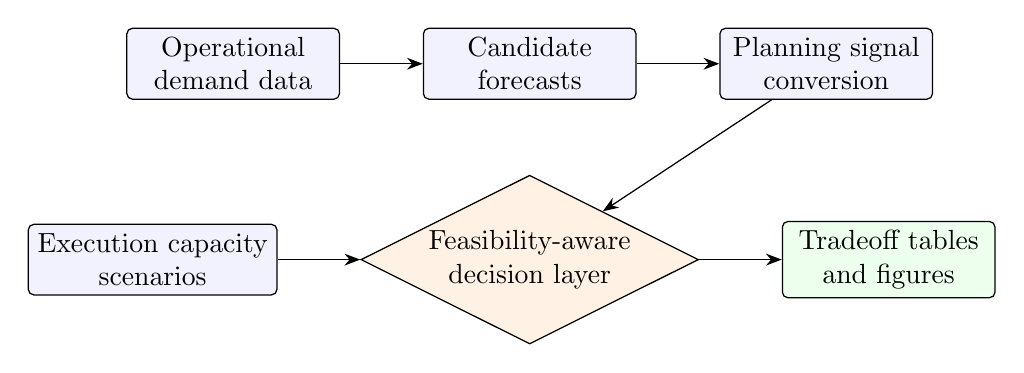
\begin{tikzpicture}[
    node distance=0.95cm and 1.05cm,
    stage/.style={
        draw,
        rounded corners=2pt,
        align=center,
        minimum width=2.7cm,
        minimum height=0.82cm,
        fill=blue!5,
        line width=0.45pt
    },
    decision/.style={
        draw,
        diamond,
        aspect=2.0,
        align=center,
        inner sep=1.2pt,
        fill=orange!10,
        line width=0.45pt
    },
    output/.style={
        draw,
        rounded corners=2pt,
        align=center,
        minimum width=2.7cm,
        minimum height=0.82cm,
        fill=green!7,
        line width=0.45pt
    },
    arrow/.style={-{Stealth[length=2.0mm]}, line width=0.45pt}
]
\node[stage] (data) {Operational\\demand data};
\node[stage, right=of data] (forecasts) {Candidate\\forecasts};
\node[stage, right=of forecasts] (signals) {Planning signal\\conversion};
\node[decision, below=of forecasts] (decision) {Feasibility-aware\\decision layer};
\node[stage, left=of decision] (capacity) {Execution capacity\\scenarios};
\node[output, right=of decision] (outputs) {Tradeoff tables\\and figures};

\draw[arrow] (data) -- (forecasts);
\draw[arrow] (forecasts) -- (signals);
\draw[arrow] (signals) -- (decision);
\draw[arrow] (capacity) -- (decision);
\draw[arrow] (decision) -- (outputs);
\end{tikzpicture}
\caption{Feasibility-aware demand-planning analysis workflow.}
\label{fig:feasibility-analysis-flowchart}
\end{figure}


% Algorithm pseudocode section for feasibility-aware model selection
% To include in main paper, add: % Algorithm pseudocode section for feasibility-aware model selection
% To include in main paper, add: % Algorithm pseudocode section for feasibility-aware model selection
% To include in main paper, add: \input{sections/algorithm_pseudocode}

\subsection{Algorithm 1: Greedy Feasibility Selector}
\label{algo:greedy-selector}

\begin{algorithm}[H]
\caption{Greedy One-Step Feasibility-Aware Selection}
\label{algo:greedy}
\begin{algorithmic}[1]
\Input{Candidate forecasts $\{\hat{y}_{i,t}^{m}\}_{m \in \mathcal{M}, t \in \mathcal{T}}$, expected losses per model}
\Input{Planning weights $\lambda_{\text{inventory}}, \lambda_{\text{volatility}}, \lambda_{\text{switch}}, \lambda_{\text{execution}}$}
\Input{Max plan-change rate $c_{\max}$ (e.g., 0.20)}
\Output{Selected forecasts and plans for each series and period}

\For{each series $i$}
    \State $z^{prev} \leftarrow \text{None}$, $x^{prev} \leftarrow 0$
    \For{each period $t$ in order}
        \State $\text{candidates} \leftarrow$ all models with available forecasts at $(i, t)$
        \State $\text{best\_score} \leftarrow +\infty$, $\text{best\_model} \leftarrow \text{None}$
        \For{each model $m \in \text{candidates}$}
            \State $\hat{x}_{i,t}^{m} \leftarrow$ forecast-to-plan conversion (e.g., inventory target)
            \State $\Delta x \leftarrow |\hat{x}_{i,t}^{m} - x^{prev}|$
            \State $\text{plan\_change\_pct} \leftarrow \Delta x / \max(|x^{prev}|, \epsilon)$
            \State $C_{i,t} \leftarrow c_{\max} \cdot |x^{prev}|$ \quad $\triangleright$ execution capacity
            \State $\text{exec\_violation} \leftarrow \max(\Delta x - C_{i,t}, 0)$
            \State $\text{base\_cost} \leftarrow$ validation-calibrated expected loss for $(i, m)$
            \State $\text{switch\_cost} \leftarrow \lambda_{\text{switch}} \cdot \mathbb{I}[m \neq z^{prev}]$
            \State $\text{score} \leftarrow \text{base\_cost} + \lambda_{\text{volatility}} \cdot \text{plan\_change\_pct}$
            \State \hspace{1.5em} $+ \lambda_{\text{execution}} \cdot \text{exec\_violation} + \text{switch\_cost}$
            \If{$\text{score} < \text{best\_score}$}
                \State $\text{best\_score} \leftarrow \text{score}$
                \State $\text{best\_model} \leftarrow m$
                \State $\text{best\_plan} \leftarrow \hat{x}_{i,t}^{m}$
            \EndIf
        \EndFor
        \State Record: $z_{i,t}^{s} \leftarrow \text{best\_model}$, $x_{i,t}^{s} \leftarrow \text{best\_plan}$
        \State $z^{prev} \leftarrow \text{best\_model}$, $x^{prev} \leftarrow \text{best\_plan}$
    \EndFor
\EndFor
\end{algorithmic}
\end{algorithm}

\subsection{Algorithm 2: Finite-Horizon DP Feasibility Selector}
\label{algo:dp-selector}

\begin{algorithm}[H]
\caption{Deterministic Finite-Horizon DP for Cumulative Loss Minimization}
\label{algo:dp}
\begin{algorithmic}[1]
\Input{Candidate forecasts $\{\hat{y}_{i,t}^{m}\}_{m \in \mathcal{M}, t \in \mathcal{T}}$, expected losses, planning weights}
\Input{Planning horizon $T$, max plan-change rate $c_{\max}$}
\Output{Optimal selected model sequence and plans for each series}

\Function{ComputeDP}{series $i$, period list $1 \ldots T$}
    \State $\text{DP}[\text{None}] \leftarrow (0.0, \text{path}=(), \text{rows}=(), \text{prev\_plan}=0)$ \quad $\triangleright$ Base case
    \For{each period $t = 1, \ldots, T$}
        \State $\text{NextDP} \leftarrow \{\}$
        \State $\text{candidates} \leftarrow$ all models at period $t$
        \For{each model $m \in \text{candidates}$}
            \State $\text{best\_prev\_state} \leftarrow \text{None}$
            \For{each $(z^{\text{prev}}, \text{state}) \in \text{DP}$}
                \State $\hat{x}_{i,t}^{m} \leftarrow$ forecast-to-plan conversion
                \State $\Delta x \leftarrow |\hat{x}_{i,t}^{m} - \text{state.prev\_plan}|$
                \State $\text{plan\_change\_pct} \leftarrow \Delta x / \max(|\text{state.prev\_plan}|, \epsilon)$
                \State $C_{i,t} \leftarrow c_{\max} \cdot |\text{state.prev\_plan}|$
                \State $\text{exec\_violation} \leftarrow \max(\Delta x - C_{i,t}, 0)$
                \State $\text{base\_cost} \leftarrow$ expected loss for $(i, m)$ at $t$
                \State $\text{stage\_cost} \leftarrow$ base\_cost + volatility + execution + switch terms
                \State $\text{new\_cost} \leftarrow \text{state.cost} + \text{stage\_cost}$
                \State $\text{candidate\_state} \leftarrow (\text{new\_cost}, \text{path}+m, \text{new\_plan})$
                \If{$\text{candidate\_state}$ dominates $\text{best\_prev\_state}$}
                    \State $\text{best\_prev\_state} \leftarrow \text{candidate\_state}$
                \EndIf
            \EndFor
            \If{$\text{best\_prev\_state} \neq \text{None}$}
                \State $\text{NextDP}[m] \leftarrow \text{best\_prev\_state}$
            \EndIf
        \EndFor
        \State $\text{DP} \leftarrow \text{NextDP}$
    \EndFor
    \State $\text{final\_state} \leftarrow \arg\min_{m} \text{DP}[m].\text{cost}$
    \State \Return paths and plans from $\text{final\_state}$
\EndFunction

\For{each series $i$}
    \State $\text{selected\_rows} \leftarrow \text{ComputeDP}(i, \text{periods})$
    \State Record selected rows with strategy label
\EndFor
\end{algorithmic}
\end{algorithm}

\subsection{Algorithm 3: Budgeted DP with Fallback}
\label{algo:budgeted-dp-selector}

\begin{algorithm}[H]
\caption{Finite-Horizon DP with Hard Switch Budget and Fallback}
\label{algo:budgeted-dp}
\begin{algorithmic}[1]
\Input{Candidate forecasts, expected losses, planning weights, max-switch budget $K$}
\Output{Selected model sequence respecting switch budget, or fallback selection}

\Function{ComputeBudgetedDP}{series $i$, period list $1 \ldots T$, budget $K$}
    \State $\text{DP}[(m, k)] \leftarrow$ state for model $m$ using $k$ switches
    \For{each period $t = 1, \ldots, T$}
        \State $\text{NextDP} \leftarrow \{\}$
        \State $\text{candidates} \leftarrow$ all models at period $t$
        \For{each model $m \in \text{candidates}$}
            \For{each $(z^{\text{prev}}, k), \text{state}) \in \text{DP}$}
                \State $k_{\text{new}} \leftarrow k + \mathbb{I}[m \neq z^{\text{prev}}]$
                \If{$k_{\text{new}} \leq K$}
                    \State Compute stage\_cost as in Algorithm \ref{algo:dp}
                    \State $\text{candidate\_state} \leftarrow$ updated DP state
                    \State $\text{NextDP}[(m, k_{\text{new}})] \leftarrow$ best state for this key
                \EndIf
            \EndFor
        \EndFor
        \State $\text{DP} \leftarrow \text{NextDP}$
        \If{$\text{DP} = \emptyset$}
            \State \textbf{break} \quad $\triangleright$ No feasible path under budget
        \EndIf
    \EndFor
    \If{$\text{DP} \neq \emptyset$}
        \State $\text{final\_state} \leftarrow \arg\min \text{DP}[*].\text{cost}$
        \State \Return paths and plans from $\text{final\_state}$
    \Else
        \State \Return $\text{IncumbentStaysFallback}(i)$ \quad $\triangleright$ Fallback policy
    \EndIf
\EndFunction

\Function{IncumbentStaysFallback}{series $i$}
    \State Select first period's lowest-cost model as incumbent $z_{\text{incumbent}}$
    \For{each period $t = 1, \ldots, T$}
        \If{$z_{\text{incumbent}}$ available at $(i, t)$}
            \State Select $z_{\text{incumbent}}$ for period $t$
        \Else
            \State Select lowest-cost available model at $(i, t)$
            \State Mark as fallback with reason: ``incumbent missing''
        \EndIf
    \EndFor
    \State \Return selected sequence with fallback annotations
\EndFunction
\end{algorithmic}
\end{algorithm}

\subsection{Methodology Notes}

The three algorithms above formalize the decision layer as follows:

\begin{itemize}
    \item \textbf{Greedy Feasibility Selector} (Algorithm \ref{algo:greedy}) makes independent one-step decisions per period. It is fast and transparent but lacks global horizon optimization.

    \item \textbf{DP Feasibility Selector} (Algorithm \ref{algo:dp}) solves the finite-horizon deterministic cumulative loss problem. State is $(z_{t-1}, \text{cost\_so\_far})$. It selects the globally optimal model sequence under the planning objective.

    \item \textbf{Budgeted DP} (Algorithm \ref{algo:budgeted-dp}) adds a hard constraint on the maximum number of model switches, useful in governance-constrained environments. If no budget-feasible path exists, the incumbent-stays fallback ensures the pipeline remains evaluable while marking the affected periods as potentially non-strict.
\end{itemize}

Key features shared across all three:
\begin{enumerate}
    \item \textbf{Deployable scoring}: Uses only validation-calibrated expected costs and forecast-implied planning signals. Test-period outcomes are never used for selection.

    \item \textbf{Consistent loss calculation}: Combines execution\_violation (absolute value, in same units as plan changes) with inventory, volatility, and switching terms using planning weights.

    \item \textbf{Execution constraint awareness}: Execution capacity $C_{i,t} = c_{\max} \cdot |x^{\text{prev}}|$ models the maximum absolute plan change the operation can absorb. Violations are penalized linearly.

    \item \textbf{Fallback safety}: The budgeted variant includes a well-defined fallback to keep pipelines evaluable even under strict switch budgets.
\end{enumerate}


\subsection{Algorithm 1: Greedy Feasibility Selector}
\label{algo:greedy-selector}

\begin{algorithm}[H]
\caption{Greedy One-Step Feasibility-Aware Selection}
\label{algo:greedy}
\begin{algorithmic}[1]
\Input{Candidate forecasts $\{\hat{y}_{i,t}^{m}\}_{m \in \mathcal{M}, t \in \mathcal{T}}$, expected losses per model}
\Input{Planning weights $\lambda_{\text{inventory}}, \lambda_{\text{volatility}}, \lambda_{\text{switch}}, \lambda_{\text{execution}}$}
\Input{Max plan-change rate $c_{\max}$ (e.g., 0.20)}
\Output{Selected forecasts and plans for each series and period}

\For{each series $i$}
    \State $z^{prev} \leftarrow \text{None}$, $x^{prev} \leftarrow 0$
    \For{each period $t$ in order}
        \State $\text{candidates} \leftarrow$ all models with available forecasts at $(i, t)$
        \State $\text{best\_score} \leftarrow +\infty$, $\text{best\_model} \leftarrow \text{None}$
        \For{each model $m \in \text{candidates}$}
            \State $\hat{x}_{i,t}^{m} \leftarrow$ forecast-to-plan conversion (e.g., inventory target)
            \State $\Delta x \leftarrow |\hat{x}_{i,t}^{m} - x^{prev}|$
            \State $\text{plan\_change\_pct} \leftarrow \Delta x / \max(|x^{prev}|, \epsilon)$
            \State $C_{i,t} \leftarrow c_{\max} \cdot |x^{prev}|$ \quad $\triangleright$ execution capacity
            \State $\text{exec\_violation} \leftarrow \max(\Delta x - C_{i,t}, 0)$
            \State $\text{base\_cost} \leftarrow$ validation-calibrated expected loss for $(i, m)$
            \State $\text{switch\_cost} \leftarrow \lambda_{\text{switch}} \cdot \mathbb{I}[m \neq z^{prev}]$
            \State $\text{score} \leftarrow \text{base\_cost} + \lambda_{\text{volatility}} \cdot \text{plan\_change\_pct}$
            \State \hspace{1.5em} $+ \lambda_{\text{execution}} \cdot \text{exec\_violation} + \text{switch\_cost}$
            \If{$\text{score} < \text{best\_score}$}
                \State $\text{best\_score} \leftarrow \text{score}$
                \State $\text{best\_model} \leftarrow m$
                \State $\text{best\_plan} \leftarrow \hat{x}_{i,t}^{m}$
            \EndIf
        \EndFor
        \State Record: $z_{i,t}^{s} \leftarrow \text{best\_model}$, $x_{i,t}^{s} \leftarrow \text{best\_plan}$
        \State $z^{prev} \leftarrow \text{best\_model}$, $x^{prev} \leftarrow \text{best\_plan}$
    \EndFor
\EndFor
\end{algorithmic}
\end{algorithm}

\subsection{Algorithm 2: Finite-Horizon DP Feasibility Selector}
\label{algo:dp-selector}

\begin{algorithm}[H]
\caption{Deterministic Finite-Horizon DP for Cumulative Loss Minimization}
\label{algo:dp}
\begin{algorithmic}[1]
\Input{Candidate forecasts $\{\hat{y}_{i,t}^{m}\}_{m \in \mathcal{M}, t \in \mathcal{T}}$, expected losses, planning weights}
\Input{Planning horizon $T$, max plan-change rate $c_{\max}$}
\Output{Optimal selected model sequence and plans for each series}

\Function{ComputeDP}{series $i$, period list $1 \ldots T$}
    \State $\text{DP}[\text{None}] \leftarrow (0.0, \text{path}=(), \text{rows}=(), \text{prev\_plan}=0)$ \quad $\triangleright$ Base case
    \For{each period $t = 1, \ldots, T$}
        \State $\text{NextDP} \leftarrow \{\}$
        \State $\text{candidates} \leftarrow$ all models at period $t$
        \For{each model $m \in \text{candidates}$}
            \State $\text{best\_prev\_state} \leftarrow \text{None}$
            \For{each $(z^{\text{prev}}, \text{state}) \in \text{DP}$}
                \State $\hat{x}_{i,t}^{m} \leftarrow$ forecast-to-plan conversion
                \State $\Delta x \leftarrow |\hat{x}_{i,t}^{m} - \text{state.prev\_plan}|$
                \State $\text{plan\_change\_pct} \leftarrow \Delta x / \max(|\text{state.prev\_plan}|, \epsilon)$
                \State $C_{i,t} \leftarrow c_{\max} \cdot |\text{state.prev\_plan}|$
                \State $\text{exec\_violation} \leftarrow \max(\Delta x - C_{i,t}, 0)$
                \State $\text{base\_cost} \leftarrow$ expected loss for $(i, m)$ at $t$
                \State $\text{stage\_cost} \leftarrow$ base\_cost + volatility + execution + switch terms
                \State $\text{new\_cost} \leftarrow \text{state.cost} + \text{stage\_cost}$
                \State $\text{candidate\_state} \leftarrow (\text{new\_cost}, \text{path}+m, \text{new\_plan})$
                \If{$\text{candidate\_state}$ dominates $\text{best\_prev\_state}$}
                    \State $\text{best\_prev\_state} \leftarrow \text{candidate\_state}$
                \EndIf
            \EndFor
            \If{$\text{best\_prev\_state} \neq \text{None}$}
                \State $\text{NextDP}[m] \leftarrow \text{best\_prev\_state}$
            \EndIf
        \EndFor
        \State $\text{DP} \leftarrow \text{NextDP}$
    \EndFor
    \State $\text{final\_state} \leftarrow \arg\min_{m} \text{DP}[m].\text{cost}$
    \State \Return paths and plans from $\text{final\_state}$
\EndFunction

\For{each series $i$}
    \State $\text{selected\_rows} \leftarrow \text{ComputeDP}(i, \text{periods})$
    \State Record selected rows with strategy label
\EndFor
\end{algorithmic}
\end{algorithm}

\subsection{Algorithm 3: Budgeted DP with Fallback}
\label{algo:budgeted-dp-selector}

\begin{algorithm}[H]
\caption{Finite-Horizon DP with Hard Switch Budget and Fallback}
\label{algo:budgeted-dp}
\begin{algorithmic}[1]
\Input{Candidate forecasts, expected losses, planning weights, max-switch budget $K$}
\Output{Selected model sequence respecting switch budget, or fallback selection}

\Function{ComputeBudgetedDP}{series $i$, period list $1 \ldots T$, budget $K$}
    \State $\text{DP}[(m, k)] \leftarrow$ state for model $m$ using $k$ switches
    \For{each period $t = 1, \ldots, T$}
        \State $\text{NextDP} \leftarrow \{\}$
        \State $\text{candidates} \leftarrow$ all models at period $t$
        \For{each model $m \in \text{candidates}$}
            \For{each $(z^{\text{prev}}, k), \text{state}) \in \text{DP}$}
                \State $k_{\text{new}} \leftarrow k + \mathbb{I}[m \neq z^{\text{prev}}]$
                \If{$k_{\text{new}} \leq K$}
                    \State Compute stage\_cost as in Algorithm \ref{algo:dp}
                    \State $\text{candidate\_state} \leftarrow$ updated DP state
                    \State $\text{NextDP}[(m, k_{\text{new}})] \leftarrow$ best state for this key
                \EndIf
            \EndFor
        \EndFor
        \State $\text{DP} \leftarrow \text{NextDP}$
        \If{$\text{DP} = \emptyset$}
            \State \textbf{break} \quad $\triangleright$ No feasible path under budget
        \EndIf
    \EndFor
    \If{$\text{DP} \neq \emptyset$}
        \State $\text{final\_state} \leftarrow \arg\min \text{DP}[*].\text{cost}$
        \State \Return paths and plans from $\text{final\_state}$
    \Else
        \State \Return $\text{IncumbentStaysFallback}(i)$ \quad $\triangleright$ Fallback policy
    \EndIf
\EndFunction

\Function{IncumbentStaysFallback}{series $i$}
    \State Select first period's lowest-cost model as incumbent $z_{\text{incumbent}}$
    \For{each period $t = 1, \ldots, T$}
        \If{$z_{\text{incumbent}}$ available at $(i, t)$}
            \State Select $z_{\text{incumbent}}$ for period $t$
        \Else
            \State Select lowest-cost available model at $(i, t)$
            \State Mark as fallback with reason: ``incumbent missing''
        \EndIf
    \EndFor
    \State \Return selected sequence with fallback annotations
\EndFunction
\end{algorithmic}
\end{algorithm}

\subsection{Methodology Notes}

The three algorithms above formalize the decision layer as follows:

\begin{itemize}
    \item \textbf{Greedy Feasibility Selector} (Algorithm \ref{algo:greedy}) makes independent one-step decisions per period. It is fast and transparent but lacks global horizon optimization.

    \item \textbf{DP Feasibility Selector} (Algorithm \ref{algo:dp}) solves the finite-horizon deterministic cumulative loss problem. State is $(z_{t-1}, \text{cost\_so\_far})$. It selects the globally optimal model sequence under the planning objective.

    \item \textbf{Budgeted DP} (Algorithm \ref{algo:budgeted-dp}) adds a hard constraint on the maximum number of model switches, useful in governance-constrained environments. If no budget-feasible path exists, the incumbent-stays fallback ensures the pipeline remains evaluable while marking the affected periods as potentially non-strict.
\end{itemize}

Key features shared across all three:
\begin{enumerate}
    \item \textbf{Deployable scoring}: Uses only validation-calibrated expected costs and forecast-implied planning signals. Test-period outcomes are never used for selection.

    \item \textbf{Consistent loss calculation}: Combines execution\_violation (absolute value, in same units as plan changes) with inventory, volatility, and switching terms using planning weights.

    \item \textbf{Execution constraint awareness}: Execution capacity $C_{i,t} = c_{\max} \cdot |x^{\text{prev}}|$ models the maximum absolute plan change the operation can absorb. Violations are penalized linearly.

    \item \textbf{Fallback safety}: The budgeted variant includes a well-defined fallback to keep pipelines evaluable even under strict switch budgets.
\end{enumerate}


\subsection{Algorithm 1: Greedy Feasibility Selector}
\label{algo:greedy-selector}

\begin{algorithm}[H]
\caption{Greedy One-Step Feasibility-Aware Selection}
\label{algo:greedy}
\begin{algorithmic}[1]
\Input{Candidate forecasts $\{\hat{y}_{i,t}^{m}\}_{m \in \mathcal{M}, t \in \mathcal{T}}$, expected losses per model}
\Input{Planning weights $\lambda_{\text{inventory}}, \lambda_{\text{volatility}}, \lambda_{\text{switch}}, \lambda_{\text{execution}}$}
\Input{Max plan-change rate $c_{\max}$ (e.g., 0.20)}
\Output{Selected forecasts and plans for each series and period}

\For{each series $i$}
    \State $z^{prev} \leftarrow \text{None}$, $x^{prev} \leftarrow 0$
    \For{each period $t$ in order}
        \State $\text{candidates} \leftarrow$ all models with available forecasts at $(i, t)$
        \State $\text{best\_score} \leftarrow +\infty$, $\text{best\_model} \leftarrow \text{None}$
        \For{each model $m \in \text{candidates}$}
            \State $\hat{x}_{i,t}^{m} \leftarrow$ forecast-to-plan conversion (e.g., inventory target)
            \State $\Delta x \leftarrow |\hat{x}_{i,t}^{m} - x^{prev}|$
            \State $\text{plan\_change\_pct} \leftarrow \Delta x / \max(|x^{prev}|, \epsilon)$
            \State $C_{i,t} \leftarrow c_{\max} \cdot |x^{prev}|$ \quad $\triangleright$ execution capacity
            \State $\text{exec\_violation} \leftarrow \max(\Delta x - C_{i,t}, 0)$
            \State $\text{base\_cost} \leftarrow$ validation-calibrated expected loss for $(i, m)$
            \State $\text{switch\_cost} \leftarrow \lambda_{\text{switch}} \cdot \mathbb{I}[m \neq z^{prev}]$
            \State $\text{score} \leftarrow \text{base\_cost} + \lambda_{\text{volatility}} \cdot \text{plan\_change\_pct}$
            \State \hspace{1.5em} $+ \lambda_{\text{execution}} \cdot \text{exec\_violation} + \text{switch\_cost}$
            \If{$\text{score} < \text{best\_score}$}
                \State $\text{best\_score} \leftarrow \text{score}$
                \State $\text{best\_model} \leftarrow m$
                \State $\text{best\_plan} \leftarrow \hat{x}_{i,t}^{m}$
            \EndIf
        \EndFor
        \State Record: $z_{i,t}^{s} \leftarrow \text{best\_model}$, $x_{i,t}^{s} \leftarrow \text{best\_plan}$
        \State $z^{prev} \leftarrow \text{best\_model}$, $x^{prev} \leftarrow \text{best\_plan}$
    \EndFor
\EndFor
\end{algorithmic}
\end{algorithm}

\subsection{Algorithm 2: Finite-Horizon DP Feasibility Selector}
\label{algo:dp-selector}

\begin{algorithm}[H]
\caption{Deterministic Finite-Horizon DP for Cumulative Loss Minimization}
\label{algo:dp}
\begin{algorithmic}[1]
\Input{Candidate forecasts $\{\hat{y}_{i,t}^{m}\}_{m \in \mathcal{M}, t \in \mathcal{T}}$, expected losses, planning weights}
\Input{Planning horizon $T$, max plan-change rate $c_{\max}$}
\Output{Optimal selected model sequence and plans for each series}

\Function{ComputeDP}{series $i$, period list $1 \ldots T$}
    \State $\text{DP}[\text{None}] \leftarrow (0.0, \text{path}=(), \text{rows}=(), \text{prev\_plan}=0)$ \quad $\triangleright$ Base case
    \For{each period $t = 1, \ldots, T$}
        \State $\text{NextDP} \leftarrow \{\}$
        \State $\text{candidates} \leftarrow$ all models at period $t$
        \For{each model $m \in \text{candidates}$}
            \State $\text{best\_prev\_state} \leftarrow \text{None}$
            \For{each $(z^{\text{prev}}, \text{state}) \in \text{DP}$}
                \State $\hat{x}_{i,t}^{m} \leftarrow$ forecast-to-plan conversion
                \State $\Delta x \leftarrow |\hat{x}_{i,t}^{m} - \text{state.prev\_plan}|$
                \State $\text{plan\_change\_pct} \leftarrow \Delta x / \max(|\text{state.prev\_plan}|, \epsilon)$
                \State $C_{i,t} \leftarrow c_{\max} \cdot |\text{state.prev\_plan}|$
                \State $\text{exec\_violation} \leftarrow \max(\Delta x - C_{i,t}, 0)$
                \State $\text{base\_cost} \leftarrow$ expected loss for $(i, m)$ at $t$
                \State $\text{stage\_cost} \leftarrow$ base\_cost + volatility + execution + switch terms
                \State $\text{new\_cost} \leftarrow \text{state.cost} + \text{stage\_cost}$
                \State $\text{candidate\_state} \leftarrow (\text{new\_cost}, \text{path}+m, \text{new\_plan})$
                \If{$\text{candidate\_state}$ dominates $\text{best\_prev\_state}$}
                    \State $\text{best\_prev\_state} \leftarrow \text{candidate\_state}$
                \EndIf
            \EndFor
            \If{$\text{best\_prev\_state} \neq \text{None}$}
                \State $\text{NextDP}[m] \leftarrow \text{best\_prev\_state}$
            \EndIf
        \EndFor
        \State $\text{DP} \leftarrow \text{NextDP}$
    \EndFor
    \State $\text{final\_state} \leftarrow \arg\min_{m} \text{DP}[m].\text{cost}$
    \State \Return paths and plans from $\text{final\_state}$
\EndFunction

\For{each series $i$}
    \State $\text{selected\_rows} \leftarrow \text{ComputeDP}(i, \text{periods})$
    \State Record selected rows with strategy label
\EndFor
\end{algorithmic}
\end{algorithm}

\subsection{Algorithm 3: Budgeted DP with Fallback}
\label{algo:budgeted-dp-selector}

\begin{algorithm}[H]
\caption{Finite-Horizon DP with Hard Switch Budget and Fallback}
\label{algo:budgeted-dp}
\begin{algorithmic}[1]
\Input{Candidate forecasts, expected losses, planning weights, max-switch budget $K$}
\Output{Selected model sequence respecting switch budget, or fallback selection}

\Function{ComputeBudgetedDP}{series $i$, period list $1 \ldots T$, budget $K$}
    \State $\text{DP}[(m, k)] \leftarrow$ state for model $m$ using $k$ switches
    \For{each period $t = 1, \ldots, T$}
        \State $\text{NextDP} \leftarrow \{\}$
        \State $\text{candidates} \leftarrow$ all models at period $t$
        \For{each model $m \in \text{candidates}$}
            \For{each $(z^{\text{prev}}, k), \text{state}) \in \text{DP}$}
                \State $k_{\text{new}} \leftarrow k + \mathbb{I}[m \neq z^{\text{prev}}]$
                \If{$k_{\text{new}} \leq K$}
                    \State Compute stage\_cost as in Algorithm \ref{algo:dp}
                    \State $\text{candidate\_state} \leftarrow$ updated DP state
                    \State $\text{NextDP}[(m, k_{\text{new}})] \leftarrow$ best state for this key
                \EndIf
            \EndFor
        \EndFor
        \State $\text{DP} \leftarrow \text{NextDP}$
        \If{$\text{DP} = \emptyset$}
            \State \textbf{break} \quad $\triangleright$ No feasible path under budget
        \EndIf
    \EndFor
    \If{$\text{DP} \neq \emptyset$}
        \State $\text{final\_state} \leftarrow \arg\min \text{DP}[*].\text{cost}$
        \State \Return paths and plans from $\text{final\_state}$
    \Else
        \State \Return $\text{IncumbentStaysFallback}(i)$ \quad $\triangleright$ Fallback policy
    \EndIf
\EndFunction

\Function{IncumbentStaysFallback}{series $i$}
    \State Select first period's lowest-cost model as incumbent $z_{\text{incumbent}}$
    \For{each period $t = 1, \ldots, T$}
        \If{$z_{\text{incumbent}}$ available at $(i, t)$}
            \State Select $z_{\text{incumbent}}$ for period $t$
        \Else
            \State Select lowest-cost available model at $(i, t)$
            \State Mark as fallback with reason: ``incumbent missing''
        \EndIf
    \EndFor
    \State \Return selected sequence with fallback annotations
\EndFunction
\end{algorithmic}
\end{algorithm}

\subsection{Methodology Notes}

The three algorithms above formalize the decision layer as follows:

\begin{itemize}
    \item \textbf{Greedy Feasibility Selector} (Algorithm \ref{algo:greedy}) makes independent one-step decisions per period. It is fast and transparent but lacks global horizon optimization.

    \item \textbf{DP Feasibility Selector} (Algorithm \ref{algo:dp}) solves the finite-horizon deterministic cumulative loss problem. State is $(z_{t-1}, \text{cost\_so\_far})$. It selects the globally optimal model sequence under the planning objective.

    \item \textbf{Budgeted DP} (Algorithm \ref{algo:budgeted-dp}) adds a hard constraint on the maximum number of model switches, useful in governance-constrained environments. If no budget-feasible path exists, the incumbent-stays fallback ensures the pipeline remains evaluable while marking the affected periods as potentially non-strict.
\end{itemize}

Key features shared across all three:
\begin{enumerate}
    \item \textbf{Deployable scoring}: Uses only validation-calibrated expected costs and forecast-implied planning signals. Test-period outcomes are never used for selection.

    \item \textbf{Consistent loss calculation}: Combines execution\_violation (absolute value, in same units as plan changes) with inventory, volatility, and switching terms using planning weights.

    \item \textbf{Execution constraint awareness}: Execution capacity $C_{i,t} = c_{\max} \cdot |x^{\text{prev}}|$ models the maximum absolute plan change the operation can absorb. Violations are penalized linearly.

    \item \textbf{Fallback safety}: The budgeted variant includes a well-defined fallback to keep pipelines evaluable even under strict switch budgets.
\end{enumerate}

\section{Experimental Setup}

\subsection{Datasets}

This subsection is a placeholder for public demand datasets. Candidate datasets include retail, grocery, store-item, and service demand tables with enough history to evaluate rolling planning decisions.

M5 is used as a large-scale hierarchical robustness dataset. It is not treated as a separate forecasting leaderboard task. The M5 robustness analysis uses manually provided local files, converts the wide daily sales table into a long item-store panel, and evaluates whether the Favorita accuracy-feasibility tradeoff persists under larger scale, hierarchy, and intermittent demand.

\subsection{Forecasting Models}

This subsection will describe candidate forecasting models. Initial models may include transparent baselines such as last-value forecasts, rolling averages, seasonal naive forecasts, and later machine learning models.

\subsection{Decision Strategies}

This subsection will describe decision strategies, including forecast pass-through, hard model selection, soft ensemble composition, and stability-aware selection with switching or volatility penalties.

The baseline comparison includes BestAccuracy, Family Best, Feasibility-Aware, Stability-Aware, Simple Ensemble, Best Inventory Cost, Best Stability, and an Oracle upper bound. The Oracle strategy may use realized test-period outcomes and is therefore non-deployable; it is included only as a diagnostic upper bound.

The improved method comparison adds feasibility-aware smoothed planning and feasibility-aware ensemble strategies. Fixed-alpha smoothing, scenario-based alpha smoothing, and utility-based alpha smoothing are evaluated as interpretable gradual-adaptation policies. Utility-based alpha is selected with blocked validation folds to reduce overfitting to a single validation period. Feasibility-aware ensembles include inverse-accuracy weighting, inverse-operational-loss weighting, and a constrained validation-grid ensemble with nonnegative weights that sum to one.

\subsection{Evaluation Metrics}

This subsection will define forecast metrics, inventory metrics, stability metrics, execution adaptation metrics, and the weighted planning utility objective used in the experiments.

Normalized planning loss is reported relative to the accuracy-first BestAccuracy baseline within the same run mode and split. Raw WAPE, inventory cost, planning volatility, execution penalty, violation rate, switch count, and raw total planning loss remain visible in the result tables.

The improved method analysis also reports the maximum period plan change, normalized inventory component, normalized volatility component, normalized execution component, normalized switch component, rank by normalized total loss, rank by WAPE, rank by execution penalty, and gap to the non-deployable Oracle diagnostic.

\subsection{Execution Capacity Scenarios}

This subsection will describe execution capacity stress tests. These scenarios evaluate how planning strategies behave when downstream operations can absorb only limited period-to-period plan changes.

DataCo is used to construct data-informed execution-risk scenarios rather than to directly estimate the exact economic cost of execution violations in the demand-planning datasets. When DataCo late-delivery anchors are unavailable, the pipeline records fallback usage and applies configured default scenario values.

The M5 robustness pipeline reuses the same DataCo-informed execution scenarios when the generated scenario table is available. If the generated table is unavailable, configured fallback scenarios are used and the run log records this explicitly.

\subsection{M5 Robustness Design}

This subsection is a placeholder for the M5 robustness design. The planned analysis includes large-scale replication at item-store level, hierarchy sensitivity across item-store, department-store, and category-store grains, intermittent-demand stress tests, and DataCo-informed execution scenario robustness.

\subsection{Policy and Context Drift Scenarios}

This subsection will describe policy and context drift scenarios, such as changes in service-level targets, shortage costs, lead times, or execution capacity.

\section{Results}

This section is a placeholder. No final experimental results are reported at this stage.

\subsection{Model Heterogeneity Results}

Placeholder for results showing how candidate forecasting models differ across planning units, time periods, or demand regimes.

\subsection{Accuracy versus Inventory Cost}

Placeholder for analysis comparing forecast accuracy improvements against inventory holding and shortage costs.

\subsection{Accuracy versus Planning Volatility}

Placeholder for analysis showing whether more accurate forecasts create larger planning signal changes.

\subsection{Execution Capacity Stress Test}

Placeholder for stress-test results showing when planning signals exceed execution capacity.

\subsection{Policy Drift Results}

Placeholder for results under changing service-level targets, shortage costs, lead times, or execution capacity.

\subsection{Ablation Study}

Placeholder for ablation results isolating the contribution of stability penalties, switching penalties, execution penalties, and safety stock assumptions.

\section{Discussion}

This section will interpret the empirical findings and explain when stability-aware decision layers improve operational planning utility. It will also discuss limitations, generalizability, and implications for planning system design.

\section{Conclusion}

Forecast accuracy remains central to demand planning, but it is not sufficient for deployment. Operational systems execute planning signals, not forecast-error tables. A model that improves WAPE can still create unstable targets, frequent adjustments, switching burden, or execution violations that make the plan less deployable.

This paper formulates forecast-driven demand planning as feasibility-constrained model selection. The framework evaluates candidate strategies using inventory exposure, planning volatility, switching burden, and execution-capacity violations alongside forecast accuracy. DataCo provides an empirical anchor for execution-risk sensitivity, Favorita provides the main forecast-to-plan proof of concept, and M5 provides hierarchical robustness evidence.

The current results show that execution-risk-sensitive objectives can reorder deployable strategy rankings. They also show that the preferred deployable method depends on execution scenario, planning granularity, and demand intermittency. This does not imply that any single feasibility-aware method universally dominates. It supports the narrower and more operationally useful conclusion that feasibility must be evaluated explicitly when forecasting models are selected for planning systems.

The manuscript is intentionally structured as a living draft. Additional Walmart and Rossmann robustness experiments, richer execution-cost calibration, and enterprise workflow evidence can be incorporated without changing the core argument: accurate forecasts become operationally valuable only when they can be converted into feasible plans.

\appendix

\section{Additional Robustness Assets}

This appendix is reserved for supplementary tables and figures that may be moved out of the main text during a later submission-preparation pass. Candidate appendix materials include full weight-sensitivity grids, execution-capacity stress tests, Pareto summaries, Favorita sample-size robustness outputs, Walmart stress-window outputs, Walmart weekly-cadence outputs, and additional Rossmann robustness experiments if those analyses are completed.

\subsection{Walmart Supplementary Robustness Assets}

The Walmart supplementary assets report holiday and markdown stress windows, weekly cadence constraints, and the full Walmart robustness summary. These tables are included for review and should not be interpreted as final conclusions before the result patterns are audited.

\begin{table}
\centering
\caption{Walmart holiday and markdown-heavy stress-window summary.}
\label{tab:walmart-holiday-markdown-stress-by-window}
\resizebox{\textwidth}{!}{%
\begin{tabular}{llllllllllllrrrrrrrrrrrrrrrrrl}
\toprule
dataset\_name & run\_mode &           feature\_set &          experiment\_name &          window\_type & scenario\_name &                   method\_name &  deployable &                oracle\_type &  fallback\_used & fallback\_type & fallback\_reason &  WAPE &  inventory\_cost &  planning\_volatility &  execution\_penalty &  execution\_violation\_rate &  model\_switch\_count &  max\_period\_plan\_change\_pct &  normalized\_inventory\_component &  normalized\_volatility\_component &  normalized\_execution\_component &  normalized\_switch\_component &  normalized\_total\_loss &  gap\_to\_dp\_oracle &  gap\_to\_perfect\_oracle &  rank\_by\_WAPE &  rank\_by\_execution\_penalty &  rank\_by\_normalized\_total\_loss &                          strategy \\
\midrule
     walmart &    quick &          history\_only &  holiday\_markdown\_stress &               normal &      baseline &  Realized-Inventory Oracle DP &       False &  realized\_inventory\_oracle &          False &          none &            none & 0.038 &     7882543.969 &              100.331 &          11347.603 &                     0.017 &                1309 &                       1.949 &                           0.600 &                            0.107 &                           0.017 &                        0.328 &                  1.052 &             0.000 &                 -0.101 &             2 &                          1 &                              1 &    oracle\_dp\_feasibility\_selector \\
     walmart &    quick &          history\_only &  holiday\_markdown\_stress &               normal &      baseline &        Realized Demand Oracle &       False &      perfect\_demand\_oracle &          False &          none &            none & 0.000 &     4115833.731 &              194.115 &         422645.826 &                     0.123 &                   0 &                       5.459 &                           0.313 &                            0.207 &                           0.632 &                        0.000 &                  1.152 &             0.101 &                  0.000 &             1 &                          8 &                              2 &            oracle\_realized\_demand \\
     walmart &    quick &          history\_only &  holiday\_markdown\_stress &               normal &      baseline &                   Budgeted DP &        True &                       none &          False &          none &            none & 0.058 &    13550293.578 &               76.851 &          32374.772 &                     0.011 &                 102 &                       4.143 &                           1.031 &                            0.082 &                           0.048 &                        0.026 &                  1.187 &             0.135 &                  0.035 &             5 &                          4 &                              3 &  budgeted\_dp\_feasibility\_selector \\
     walmart &    quick &          history\_only &  holiday\_markdown\_stress &               normal &      baseline &                   Global Best &        True &                       none &          False &          none &            none & 0.057 &    13141862.485 &               93.868 &          66845.875 &                     0.036 &                   0 &                       3.912 &                           1.000 &                            0.100 &                           0.100 &                        0.000 &                  1.200 &             0.148 &                  0.048 &             3 &                          7 &                              4 &                 global\_best\_model \\
     walmart &    quick &          history\_only &  holiday\_markdown\_stress &               normal &      baseline &                DP Feasibility &        True &                       none &          False &          none &            none & 0.057 &    13405197.135 &               77.169 &          32123.493 &                     0.009 &                 213 &                       4.143 &                           1.020 &                            0.082 &                           0.048 &                        0.053 &                  1.204 &             0.152 &                  0.051 &             4 &                          3 &                              5 &           dp\_feasibility\_selector \\
     walmart &    quick &          history\_only &  holiday\_markdown\_stress &               normal &      baseline &          Operational Ensemble &        True &                       none &          False &          none &            none & 0.061 &    14722668.539 &               69.087 &          30977.986 &                     0.021 &                   0 &                       3.119 &                           1.120 &                            0.074 &                           0.046 &                        0.000 &                  1.240 &             0.188 &                  0.088 &             8 &                          2 &                              6 &         operational\_loss\_ensemble \\
     walmart &    quick &          history\_only &  holiday\_markdown\_stress &               normal &      baseline &               Simple Ensemble &        True &                       none &          False &          none &            none & 0.060 &    14487117.040 &               81.613 &          35526.693 &                     0.026 &                   0 &                       3.439 &                           1.102 &                            0.087 &                           0.053 &                        0.000 &                  1.242 &             0.191 &                  0.090 &             7 &                          6 &                              7 &                   simple\_ensemble \\
     walmart &    quick &          history\_only &  holiday\_markdown\_stress &               normal &      baseline &            Greedy Feasibility &        True &                       none &          False &          none &            none & 0.059 &    14063617.514 &               83.588 &          34606.282 &                     0.013 &                 186 &                       4.143 &                           1.070 &                            0.089 &                           0.052 &                        0.047 &                  1.258 &             0.206 &                  0.105 &             6 &                          5 &                              8 &       greedy\_feasibility\_selector \\
     walmart &    quick &          history\_only &  holiday\_markdown\_stress &              holiday &      baseline &                   Budgeted DP &        True &                       none &          False &          none &            none & 0.071 &     2526532.541 &                9.084 &            165.498 &                     0.005 &                   9 &                       1.542 &                           1.049 &                            0.109 &                           0.003 &                        0.026 &                  1.186 &            -0.046 &                 -2.988 &             5 &                          2 &                              1 &  budgeted\_dp\_feasibility\_selector \\
     walmart &    quick &          history\_only &  holiday\_markdown\_stress &              holiday &      baseline &                   Global Best &        True &                       none &          False &          none &            none & 0.069 &     2409172.941 &                8.350 &           5554.443 &                     0.015 &                   0 &                       0.596 &                           1.000 &                            0.100 &                           0.100 &                        0.000 &                  1.200 &            -0.032 &                 -2.974 &             3 &                          7 &                              2 &                 global\_best\_model \\
     walmart &    quick &          history\_only &  holiday\_markdown\_stress &              holiday &      baseline &            Greedy Feasibility &        True &                       none &          False &          none &            none & 0.071 &     2544462.226 &                9.379 &            165.498 &                     0.005 &                  16 &                       1.542 &                           1.056 &                            0.112 &                           0.003 &                        0.046 &                  1.217 &            -0.015 &                 -2.957 &             6 &                          2 &                              3 &       greedy\_feasibility\_selector \\
     walmart &    quick &          history\_only &  holiday\_markdown\_stress &              holiday &      baseline &                DP Feasibility &        True &                       none &          False &          none &            none & 0.071 &     2538515.091 &                8.972 &            165.498 &                     0.005 &                  19 &                       1.542 &                           1.054 &                            0.107 &                           0.003 &                        0.054 &                  1.218 &            -0.014 &                 -2.955 &             4 &                          2 &                              4 &           dp\_feasibility\_selector \\
     walmart &    quick &          history\_only &  holiday\_markdown\_stress &              holiday &      baseline &  Realized-Inventory Oracle DP &       False &  realized\_inventory\_oracle &          False &          none &            none & 0.049 &     1498825.205 &               12.500 &              6.693 &                     0.015 &                 161 &                       0.305 &                           0.622 &                            0.150 &                           0.000 &                        0.460 &                  1.232 &             0.000 &                 -2.942 &             2 &                          1 &                              5 &    oracle\_dp\_feasibility\_selector \\
     walmart &    quick &          history\_only &  holiday\_markdown\_stress &              holiday &      baseline &          Operational Ensemble &        True &                       none &          False &          none &            none & 0.075 &     2898220.998 &                6.271 &           3248.052 &                     0.020 &                   0 &                       0.500 &                           1.203 &                            0.075 &                           0.058 &                        0.000 &                  1.337 &             0.105 &                 -2.837 &             7 &                          5 &                              6 &         operational\_loss\_ensemble \\
     walmart &    quick &          history\_only &  holiday\_markdown\_stress &              holiday &      baseline &               Simple Ensemble &        True &                       none &          False &          none &            none & 0.076 &     2913711.016 &                7.524 &           3985.786 &                     0.020 &                   0 &                       0.571 &                           1.209 &                            0.090 &                           0.072 &                        0.000 &                  1.371 &             0.139 &                 -2.802 &             8 &                          6 &                              7 &                   simple\_ensemble \\
     walmart &    quick &          history\_only &  holiday\_markdown\_stress &              holiday &      baseline &        Realized Demand Oracle &       False &      perfect\_demand\_oracle &          False &          none &            none & 0.000 &      471152.918 &               29.455 &         201373.427 &                     0.197 &                   0 &                       2.337 &                           0.196 &                            0.353 &                           3.625 &                        0.000 &                  4.174 &             2.942 &                  0.000 &             1 &                          8 &                              8 &            oracle\_realized\_demand \\
     walmart &    quick &          history\_only &  holiday\_markdown\_stress &       markdown\_heavy &      baseline &  Realized-Inventory Oracle DP &       False &  realized\_inventory\_oracle &          False &          none &            none & 0.034 &     2810027.581 &               22.737 &            769.532 &                     0.006 &                 373 &                       1.363 &                           0.537 &                            0.116 &                           0.010 &                        0.460 &                  1.124 &             0.000 &                 -1.258 &             2 &                          1 &                              1 &    oracle\_dp\_feasibility\_selector \\
     walmart &    quick &          history\_only &  holiday\_markdown\_stress &       markdown\_heavy &      baseline &                   Global Best &        True &                       none &          False &          none &            none & 0.053 &     5230508.992 &               19.574 &           7686.896 &                     0.020 &                   0 &                       1.363 &                           1.000 &                            0.100 &                           0.100 &                        0.000 &                  1.200 &             0.076 &                 -1.181 &             3 &                          6 &                              2 &                 global\_best\_model \\
     walmart &    quick &          history\_only &  holiday\_markdown\_stress &       markdown\_heavy &      baseline &                   Budgeted DP &        True &                       none &          False &          none &            none & 0.054 &     5489217.130 &               22.250 &           1519.096 &                     0.009 &                  21 &                       2.383 &                           1.049 &                            0.114 &                           0.020 &                        0.026 &                  1.209 &             0.085 &                 -1.173 &             5 &                          3 &                              3 &  budgeted\_dp\_feasibility\_selector \\
     walmart &    quick &          history\_only &  holiday\_markdown\_stress &       markdown\_heavy &      baseline &                DP Feasibility &        True &                       none &          False &          none &            none & 0.054 &     5473900.394 &               22.601 &           1519.319 &                     0.011 &                  41 &                       2.383 &                           1.047 &                            0.115 &                           0.020 &                        0.051 &                  1.232 &             0.108 &                 -1.149 &             4 &                          4 &                              4 &           dp\_feasibility\_selector \\
     walmart &    quick &          history\_only &  holiday\_markdown\_stress &       markdown\_heavy &      baseline &            Greedy Feasibility &        True &                       none &          False &          none &            none & 0.055 &     5666680.051 &               23.674 &           1515.175 &                     0.009 &                  40 &                       2.383 &                           1.083 &                            0.121 &                           0.020 &                        0.049 &                  1.273 &             0.150 &                 -1.108 &             7 &                          2 &                              5 &       greedy\_feasibility\_selector \\
     walmart &    quick &          history\_only &  holiday\_markdown\_stress &       markdown\_heavy &      baseline &          Operational Ensemble &        True &                       none &          False &          none &            none & 0.055 &     5902660.054 &               16.391 &           5420.401 &                     0.017 &                   0 &                       1.681 &                           1.129 &                            0.084 &                           0.071 &                        0.000 &                  1.283 &             0.159 &                 -1.099 &             8 &                          5 &                              6 &         operational\_loss\_ensemble \\
     walmart &    quick &          history\_only &  holiday\_markdown\_stress &       markdown\_heavy &      baseline &               Simple Ensemble &        True &                       none &          False &          none &            none & 0.055 &     5813318.384 &               19.620 &           8289.496 &                     0.020 &                   0 &                       1.781 &                           1.111 &                            0.100 &                           0.108 &                        0.000 &                  1.319 &             0.196 &                 -1.062 &             6 &                          7 &                              7 &                   simple\_ensemble \\
     walmart &    quick &          history\_only &  holiday\_markdown\_stress &       markdown\_heavy &      baseline &        Realized Demand Oracle &       False &      perfect\_demand\_oracle &          False &          none &            none & 0.000 &     1703808.794 &               43.839 &         140802.552 &                     0.063 &                   0 &                       2.337 &                           0.326 &                            0.224 &                           1.832 &                        0.000 &                  2.381 &             1.258 &                  0.000 &             1 &                          8 &                              8 &            oracle\_realized\_demand \\
     walmart &    quick &          history\_only &  holiday\_markdown\_stress &  holiday\_or\_markdown &      baseline &  Realized-Inventory Oracle DP &       False &  realized\_inventory\_oracle &          False &          none &            none & 0.037 &     3988637.537 &               33.627 &            776.224 &                     0.009 &                 503 &                       1.363 &                           0.557 &                            0.126 &                           0.006 &                        0.449 &                  1.137 &             0.000 &                 -1.974 &             2 &                          1 &                              1 &    oracle\_dp\_feasibility\_selector \\
     walmart &    quick &          history\_only &  holiday\_markdown\_stress &  holiday\_or\_markdown &      baseline &                   Budgeted DP &        True &                       none &          False &          none &            none & 0.058 &     7495733.405 &               28.828 &           1519.096 &                     0.007 &                  28 &                       2.383 &                           1.046 &                            0.108 &                           0.011 &                        0.025 &                  1.190 &             0.053 &                 -1.921 &             5 &                          3 &                              2 &  budgeted\_dp\_feasibility\_selector \\
     walmart &    quick &          history\_only &  holiday\_markdown\_stress &  holiday\_or\_markdown &      baseline &                   Global Best &        True &                       none &          False &          none &            none & 0.057 &     7166517.663 &               26.749 &          13241.339 &                     0.020 &                   0 &                       1.363 &                           1.000 &                            0.100 &                           0.100 &                        0.000 &                  1.200 &             0.063 &                 -1.912 &             3 &                          7 &                              3 &                 global\_best\_model \\
     walmart &    quick &          history\_only &  holiday\_markdown\_stress &  holiday\_or\_markdown &      baseline &                DP Feasibility &        True &                       none &          False &          none &            none & 0.058 &     7487157.647 &               29.107 &           1519.319 &                     0.009 &                  58 &                       2.383 &                           1.045 &                            0.109 &                           0.011 &                        0.052 &                  1.217 &             0.080 &                 -1.895 &             4 &                          4 &                              4 &           dp\_feasibility\_selector \\
     walmart &    quick &          history\_only &  holiday\_markdown\_stress &  holiday\_or\_markdown &      baseline &            Greedy Feasibility &        True &                       none &          False &          none &            none & 0.059 &     7673529.074 &               30.578 &           1515.175 &                     0.007 &                  54 &                       2.383 &                           1.071 &                            0.114 &                           0.011 &                        0.048 &                  1.245 &             0.107 &                 -1.867 &             6 &                          2 &                              5 &       greedy\_feasibility\_selector \\
     walmart &    quick &          history\_only &  holiday\_markdown\_stress &  holiday\_or\_markdown &      baseline &          Operational Ensemble &        True &                       none &          False &          none &            none & 0.060 &     8270784.503 &               21.488 &           8630.769 &                     0.017 &                   0 &                       1.681 &                           1.154 &                            0.080 &                           0.065 &                        0.000 &                  1.300 &             0.162 &                 -1.812 &             8 &                          5 &                              6 &         operational\_loss\_ensemble \\
     walmart &    quick &          history\_only &  holiday\_markdown\_stress &  holiday\_or\_markdown &      baseline &               Simple Ensemble &        True &                       none &          False &          none &            none & 0.060 &     8179245.384 &               25.645 &          12224.613 &                     0.020 &                   0 &                       1.781 &                           1.141 &                            0.096 &                           0.092 &                        0.000 &                  1.330 &             0.192 &                 -1.782 &             7 &                          6 &                              7 &                   simple\_ensemble \\
     walmart &    quick &          history\_only &  holiday\_markdown\_stress &  holiday\_or\_markdown &      baseline &        Realized Demand Oracle &       False &      perfect\_demand\_oracle &          False &          none &            none & 0.000 &     2088018.438 &               67.527 &         340007.772 &                     0.094 &                   0 &                       2.337 &                           0.291 &                            0.252 &                           2.568 &                        0.000 &                  3.112 &             1.974 &                  0.000 &             1 &                          8 &                              8 &            oracle\_realized\_demand \\
     walmart &    quick &  history\_plus\_context &  holiday\_markdown\_stress &               normal &      baseline &  Realized-Inventory Oracle DP &       False &  realized\_inventory\_oracle &          False &          none &            none & 0.038 &     7886177.095 &               99.713 &          11333.473 &                     0.016 &                1310 &                       1.949 &                           0.598 &                            0.119 &                           0.026 &                        0.376 &                  1.120 &             0.000 &                 -0.384 &             2 &                          1 &                              1 &    oracle\_dp\_feasibility\_selector \\
     walmart &    quick &  history\_plus\_context &  holiday\_markdown\_stress &               normal &      baseline &                   Global Best &        True &                       none &          False &          none &            none & 0.057 &    13187821.306 &               83.513 &          44093.445 &                     0.031 &                   0 &                       3.111 &                           1.000 &                            0.100 &                           0.100 &                        0.000 &                  1.200 &             0.080 &                 -0.303 &             4 &                          7 &                              2 &                 global\_best\_model \\
     walmart &    quick &  history\_plus\_context &  holiday\_markdown\_stress &               normal &      baseline &                   Budgeted DP &        True &                       none &          False &          none &            none & 0.058 &    13459541.162 &               73.973 &          32276.944 &                     0.010 &                  94 &                       4.143 &                           1.021 &                            0.089 &                           0.073 &                        0.027 &                  1.209 &             0.090 &                 -0.294 &             5 &                          4 &                              3 &  budgeted\_dp\_feasibility\_selector \\
     walmart &    quick &  history\_plus\_context &  holiday\_markdown\_stress &               normal &      baseline &                DP Feasibility &        True &                       none &          False &          none &            none & 0.057 &    13343417.020 &               75.320 &          32100.649 &                     0.008 &                 178 &                       4.143 &                           1.012 &                            0.090 &                           0.073 &                        0.051 &                  1.226 &             0.106 &                 -0.277 &             3 &                          3 &                              4 &           dp\_feasibility\_selector \\
     walmart &    quick &  history\_plus\_context &  holiday\_markdown\_stress &               normal &      baseline &            Greedy Feasibility &        True &                       none &          False &          none &            none & 0.058 &    13745633.215 &               81.622 &          34053.652 &                     0.012 &                 170 &                       4.143 &                           1.042 &                            0.098 &                           0.077 &                        0.049 &                  1.266 &             0.147 &                 -0.237 &             6 &                          6 &                              5 &       greedy\_feasibility\_selector \\
     walmart &    quick &  history\_plus\_context &  holiday\_markdown\_stress &               normal &      baseline &          Operational Ensemble &        True &                       none &          False &          none &            none & 0.062 &    14824252.681 &               64.275 &          28925.468 &                     0.018 &                   0 &                       2.856 &                           1.124 &                            0.077 &                           0.066 &                        0.000 &                  1.267 &             0.147 &                 -0.236 &             8 &                          2 &                              6 &         operational\_loss\_ensemble \\
     walmart &    quick &  history\_plus\_context &  holiday\_markdown\_stress &               normal &      baseline &               Simple Ensemble &        True &                       none &          False &          none &            none & 0.060 &    14526906.431 &               79.037 &          33649.601 &                     0.026 &                   0 &                       3.272 &                           1.102 &                            0.095 &                           0.076 &                        0.000 &                  1.272 &             0.153 &                 -0.231 &             7 &                          5 &                              7 &                   simple\_ensemble \\
     walmart &    quick &  history\_plus\_context &  holiday\_markdown\_stress &               normal &      baseline &        Realized Demand Oracle &       False &      perfect\_demand\_oracle &          False &          none &            none & 0.000 &     4115833.731 &              194.115 &         422645.826 &                     0.123 &                   0 &                       5.459 &                           0.312 &                            0.232 &                           0.959 &                        0.000 &                  1.503 &             0.384 &                  0.000 &             1 &                          8 &                              8 &            oracle\_realized\_demand \\
     walmart &    quick &  history\_plus\_context &  holiday\_markdown\_stress &              holiday &      baseline &                   Budgeted DP &        True &                       none &          False &          none &            none & 0.068 &     2381644.177 &                8.621 &            165.498 &                     0.005 &                   7 &                       1.542 &                           1.068 &                            0.106 &                           0.003 &                        0.020 &                  1.196 &            -0.150 &                 -2.862 &             5 &                          1 &                              1 &  budgeted\_dp\_feasibility\_selector \\
     walmart &    quick &  history\_plus\_context &  holiday\_markdown\_stress &              holiday &      baseline &                   Global Best &        True &                       none &          False &          none &            none & 0.067 &     2230000.598 &                8.170 &           5775.458 &                     0.020 &                   0 &                       0.592 &                           1.000 &                            0.100 &                           0.100 &                        0.000 &                  1.200 &            -0.146 &                 -2.859 &             3 &                          7 &                              2 &                 global\_best\_model \\
     walmart &    quick &  history\_plus\_context &  holiday\_markdown\_stress &              holiday &      baseline &            Greedy Feasibility &        True &                       none &          False &          none &            none & 0.068 &     2375248.472 &                9.233 &            165.498 &                     0.005 &                  16 &                       1.542 &                           1.065 &                            0.113 &                           0.003 &                        0.046 &                  1.227 &            -0.120 &                 -2.832 &             4 &                          1 &                              3 &       greedy\_feasibility\_selector \\
     walmart &    quick &  history\_plus\_context &  holiday\_markdown\_stress &              holiday &      baseline &                DP Feasibility &        True &                       none &          False &          none &            none & 0.069 &     2433763.094 &                8.641 &            165.498 &                     0.005 &                  19 &                       1.542 &                           1.091 &                            0.106 &                           0.003 &                        0.054 &                  1.254 &            -0.092 &                 -2.804 &             6 &                          1 &                              4 &           dp\_feasibility\_selector \\
     walmart &    quick &  history\_plus\_context &  holiday\_markdown\_stress &              holiday &      baseline &  Realized-Inventory Oracle DP &       False &  realized\_inventory\_oracle &          False &          none &            none & 0.048 &     1455558.199 &               18.621 &            664.205 &                     0.020 &                 159 &                       5.532 &                           0.653 &                            0.228 &                           0.012 &                        0.454 &                  1.346 &             0.000 &                 -2.712 &             2 &                          4 &                              5 &    oracle\_dp\_feasibility\_selector \\
     walmart &    quick &  history\_plus\_context &  holiday\_markdown\_stress &              holiday &      baseline &          Operational Ensemble &        True &                       none &          False &          none &            none & 0.075 &     2852336.130 &                5.849 &           3151.115 &                     0.015 &                   0 &                       0.493 &                           1.279 &                            0.072 &                           0.055 &                        0.000 &                  1.405 &             0.059 &                 -2.653 &             7 &                          5 &                              6 &         operational\_loss\_ensemble \\
     walmart &    quick &  history\_plus\_context &  holiday\_markdown\_stress &              holiday &      baseline &               Simple Ensemble &        True &                       none &          False &          none &            none & 0.075 &     2881817.402 &                7.018 &           3901.335 &                     0.015 &                   0 &                       0.553 &                           1.292 &                            0.086 &                           0.068 &                        0.000 &                  1.446 &             0.099 &                 -2.613 &             8 &                          6 &                              7 &                   simple\_ensemble \\
     walmart &    quick &  history\_plus\_context &  holiday\_markdown\_stress &              holiday &      baseline &        Realized Demand Oracle &       False &      perfect\_demand\_oracle &          False &          none &            none & 0.000 &      471152.918 &               29.455 &         201373.427 &                     0.197 &                   0 &                       2.337 &                           0.211 &                            0.361 &                           3.487 &                        0.000 &                  4.059 &             2.712 &                  0.000 &             1 &                          8 &                              8 &            oracle\_realized\_demand \\
     walmart &    quick &  history\_plus\_context &  holiday\_markdown\_stress &       markdown\_heavy &      baseline &  Realized-Inventory Oracle DP &       False &  realized\_inventory\_oracle &          False &          none &            none & 0.033 &     2771954.257 &               27.796 &            887.717 &                     0.008 &                 378 &                       5.532 &                           0.540 &                            0.141 &                           0.013 &                        0.455 &                  1.150 &             0.000 &                 -1.447 &             2 &                          1 &                              1 &    oracle\_dp\_feasibility\_selector \\
     walmart &    quick &  history\_plus\_context &  holiday\_markdown\_stress &       markdown\_heavy &      baseline &                   Global Best &        True &                       none &          False &          none &            none & 0.054 &     5131615.701 &               19.689 &           6896.885 &                     0.022 &                   0 &                       1.053 &                           1.000 &                            0.100 &                           0.100 &                        0.000 &                  1.200 &             0.050 &                 -1.396 &             5 &                          6 &                              2 &                 global\_best\_model \\
     walmart &    quick &  history\_plus\_context &  holiday\_markdown\_stress &       markdown\_heavy &      baseline &                   Budgeted DP &        True &                       none &          False &          none &            none & 0.054 &     5417599.275 &               22.228 &           1519.096 &                     0.009 &                  27 &                       2.383 &                           1.056 &                            0.113 &                           0.022 &                        0.033 &                  1.223 &             0.074 &                 -1.373 &             4 &                          3 &                              3 &  budgeted\_dp\_feasibility\_selector \\
     walmart &    quick &  history\_plus\_context &  holiday\_markdown\_stress &       markdown\_heavy &      baseline &                DP Feasibility &        True &                       none &          False &          none &            none & 0.054 &     5366712.339 &               23.039 &           1519.319 &                     0.011 &                  45 &                       2.383 &                           1.046 &                            0.117 &                           0.022 &                        0.054 &                  1.239 &             0.089 &                 -1.357 &             3 &                          4 &                              4 &           dp\_feasibility\_selector \\
     walmart &    quick &  history\_plus\_context &  holiday\_markdown\_stress &       markdown\_heavy &      baseline &            Greedy Feasibility &        True &                       none &          False &          none &            none & 0.055 &     5476698.433 &               23.535 &           1515.175 &                     0.009 &                  38 &                       2.383 &                           1.067 &                            0.120 &                           0.022 &                        0.046 &                  1.255 &             0.105 &                 -1.342 &             7 &                          2 &                              5 &       greedy\_feasibility\_selector \\
     walmart &    quick &  history\_plus\_context &  holiday\_markdown\_stress &       markdown\_heavy &      baseline &          Operational Ensemble &        True &                       none &          False &          none &            none & 0.056 &     5873531.341 &               15.690 &           4936.498 &                     0.023 &                   0 &                       1.031 &                           1.145 &                            0.080 &                           0.072 &                        0.000 &                  1.296 &             0.146 &                 -1.300 &             8 &                          5 &                              6 &         operational\_loss\_ensemble \\
     walmart &    quick &  history\_plus\_context &  holiday\_markdown\_stress &       markdown\_heavy &      baseline &               Simple Ensemble &        True &                       none &          False &          none &            none & 0.055 &     5772229.904 &               19.067 &           8163.536 &                     0.023 &                   0 &                       1.248 &                           1.125 &                            0.097 &                           0.118 &                        0.000 &                  1.340 &             0.190 &                 -1.256 &             6 &                          7 &                              7 &                   simple\_ensemble \\
     walmart &    quick &  history\_plus\_context &  holiday\_markdown\_stress &       markdown\_heavy &      baseline &        Realized Demand Oracle &       False &      perfect\_demand\_oracle &          False &          none &            none & 0.000 &     1703808.794 &               43.839 &         140802.552 &                     0.063 &                   0 &                       2.337 &                           0.332 &                            0.223 &                           2.042 &                        0.000 &                  2.596 &             1.447 &                  0.000 &             1 &                          8 &                              8 &            oracle\_realized\_demand \\
     walmart &    quick &  history\_plus\_context &  holiday\_markdown\_stress &  holiday\_or\_markdown &      baseline &  Realized-Inventory Oracle DP &       False &  realized\_inventory\_oracle &          False &          none &            none & 0.037 &     3936430.047 &               39.330 &            894.409 &                     0.010 &                 507 &                       5.532 &                           0.564 &                            0.150 &                           0.007 &                        0.441 &                  1.162 &             0.000 &                 -2.170 &             2 &                          1 &                              1 &    oracle\_dp\_feasibility\_selector \\
     walmart &    quick &  history\_plus\_context &  holiday\_markdown\_stress &  holiday\_or\_markdown &      baseline &                   Budgeted DP &        True &                       none &          False &          none &            none & 0.058 &     7325834.828 &               28.480 &           1519.096 &                     0.007 &                  34 &                       2.383 &                           1.050 &                            0.108 &                           0.012 &                        0.030 &                  1.200 &             0.038 &                 -2.132 &             4 &                          3 &                              2 &  budgeted\_dp\_feasibility\_selector \\
     walmart &    quick &  history\_plus\_context &  holiday\_markdown\_stress &  holiday\_or\_markdown &      baseline &                   Global Best &        True &                       none &          False &          none &            none & 0.058 &     6979417.984 &               26.304 &          12248.638 &                     0.021 &                   0 &                       1.053 &                           1.000 &                            0.100 &                           0.100 &                        0.000 &                  1.200 &             0.038 &                 -2.132 &             5 &                          7 &                              3 &                 global\_best\_model \\
     walmart &    quick &  history\_plus\_context &  holiday\_markdown\_stress &  holiday\_or\_markdown &      baseline &                DP Feasibility &        True &                       none &          False &          none &            none & 0.057 &     7320432.320 &               29.196 &           1519.319 &                     0.009 &                  63 &                       2.383 &                           1.049 &                            0.111 &                           0.012 &                        0.055 &                  1.227 &             0.065 &                 -2.105 &             3 &                          4 &                              4 &           dp\_feasibility\_selector \\
     walmart &    quick &  history\_plus\_context &  holiday\_markdown\_stress &  holiday\_or\_markdown &      baseline &            Greedy Feasibility &        True &                       none &          False &          none &            none & 0.058 &     7369352.031 &               30.300 &           1515.175 &                     0.007 &                  52 &                       2.383 &                           1.056 &                            0.115 &                           0.012 &                        0.045 &                  1.229 &             0.067 &                 -2.103 &             6 &                          2 &                              5 &       greedy\_feasibility\_selector \\
     walmart &    quick &  history\_plus\_context &  holiday\_markdown\_stress &  holiday\_or\_markdown &      baseline &          Operational Ensemble &        True &                       none &          False &          none &            none & 0.060 &     8222608.763 &               20.628 &           8058.002 &                     0.021 &                   0 &                       1.031 &                           1.178 &                            0.078 &                           0.066 &                        0.000 &                  1.322 &             0.161 &                 -2.009 &             8 &                          5 &                              6 &         operational\_loss\_ensemble \\
     walmart &    quick &  history\_plus\_context &  holiday\_markdown\_stress &  holiday\_or\_markdown &      baseline &               Simple Ensemble &        True &                       none &          False &          none &            none & 0.060 &     8123692.535 &               25.041 &          12064.871 &                     0.022 &                   0 &                       1.248 &                           1.164 &                            0.095 &                           0.098 &                        0.000 &                  1.358 &             0.196 &                 -1.974 &             7 &                          6 &                              7 &                   simple\_ensemble \\
     walmart &    quick &  history\_plus\_context &  holiday\_markdown\_stress &  holiday\_or\_markdown &      baseline &        Realized Demand Oracle &       False &      perfect\_demand\_oracle &          False &          none &            none & 0.000 &     2088018.438 &               67.527 &         340007.772 &                     0.094 &                   0 &                       2.337 &                           0.299 &                            0.257 &                           2.776 &                        0.000 &                  3.332 &             2.170 &                  0.000 &             1 &                          8 &                              8 &            oracle\_realized\_demand \\
\bottomrule
\end{tabular}
}

\end{table}

\begin{table}
\centering
\caption{Walmart weekly cadence constraint summary.}
\label{tab:walmart-weekly-cadence-constraints}
\resizebox{\textwidth}{!}{%
\begin{tabular}{llllllllllllrrrrrrrrrrrrrrrrrl}
\toprule
dataset\_name & run\_mode &           feature\_set &             experiment\_name & window\_type &   scenario\_name &                   method\_name &  deployable &                oracle\_type &  fallback\_used & fallback\_type & fallback\_reason &  WAPE &  inventory\_cost &  planning\_volatility &  execution\_penalty &  execution\_violation\_rate &  model\_switch\_count &  max\_period\_plan\_change\_pct &  normalized\_inventory\_component &  normalized\_volatility\_component &  normalized\_execution\_component &  normalized\_switch\_component &  normalized\_total\_loss &  gap\_to\_dp\_oracle &  gap\_to\_perfect\_oracle &  rank\_by\_WAPE &  rank\_by\_execution\_penalty &  rank\_by\_normalized\_total\_loss &                          strategy \\
\midrule
     walmart &    quick &          history\_only &  weekly\_cadence\_constraints &         all &  weekly\_cadence &  Realized-Inventory Oracle DP &       False &  realized\_inventory\_oracle &          False &          none &            none & 0.038 &    11871181.507 &              133.958 &          12123.827 &                     0.014 &                1812 &                       1.949 &                           0.585 &                            0.111 &                           0.015 &                        0.414 &                  1.124 &             0.000 &                 -0.350 &             2 &                          1 &                              1 &    oracle\_dp\_feasibility\_selector \\
     walmart &    quick &          history\_only &  weekly\_cadence\_constraints &         all &  weekly\_cadence &                   Global Best &        True &                       none &          False &          none &            none & 0.057 &    20308380.148 &              120.617 &          80087.213 &                     0.031 &                   0 &                       3.912 &                           1.000 &                            0.100 &                           0.100 &                        0.000 &                  1.200 &             0.076 &                 -0.275 &             3 &                          5 &                              2 &                 global\_best\_model \\
     walmart &    quick &          history\_only &  weekly\_cadence\_constraints &         all &  weekly\_cadence &                   Budgeted DP &        True &                       none &          False &          none &            none & 0.058 &    21051365.157 &              111.252 &          77726.400 &                     0.017 &                 118 &                       4.143 &                           1.037 &                            0.092 &                           0.097 &                        0.027 &                  1.253 &             0.128 &                 -0.222 &             5 &                          4 &                              3 &  budgeted\_dp\_feasibility\_selector \\
     walmart &    quick &          history\_only &  weekly\_cadence\_constraints &         all &  weekly\_cadence &          Operational Ensemble &        True &                       none &          False &          none &            none & 0.061 &    22993453.042 &               90.574 &          39608.755 &                     0.020 &                   0 &                       3.119 &                           1.132 &                            0.075 &                           0.049 &                        0.000 &                  1.257 &             0.132 &                 -0.218 &             8 &                          2 &                              4 &         operational\_loss\_ensemble \\
     walmart &    quick &          history\_only &  weekly\_cadence\_constraints &         all &  weekly\_cadence &               Simple Ensemble &        True &                       none &          False &          none &            none & 0.060 &    22666362.424 &              107.258 &          47751.305 &                     0.024 &                   0 &                       3.439 &                           1.116 &                            0.089 &                           0.060 &                        0.000 &                  1.265 &             0.140 &                 -0.210 &             7 &                          3 &                              5 &                   simple\_ensemble \\
     walmart &    quick &          history\_only &  weekly\_cadence\_constraints &         all &  weekly\_cadence &                DP Feasibility &        True &                       none &          False &          none &            none & 0.058 &    20957913.234 &              111.816 &          97687.589 &                     0.017 &                 225 &                       4.143 &                           1.032 &                            0.093 &                           0.122 &                        0.051 &                  1.298 &             0.174 &                 -0.177 &             4 &                          6 &                              6 &           dp\_feasibility\_selector \\
     walmart &    quick &          history\_only &  weekly\_cadence\_constraints &         all &  weekly\_cadence &            Greedy Feasibility &        True &                       none &          False &          none &            none & 0.059 &    21749818.252 &              119.061 &         128611.004 &                     0.017 &                 213 &                       4.143 &                           1.071 &                            0.099 &                           0.161 &                        0.049 &                  1.379 &             0.254 &                 -0.096 &             6 &                          7 &                              7 &       greedy\_feasibility\_selector \\
     walmart &    quick &          history\_only &  weekly\_cadence\_constraints &         all &  weekly\_cadence &        Realized Demand Oracle &       False &      perfect\_demand\_oracle &          False &          none &            none & 0.000 &     6203852.169 &              261.641 &         762653.598 &                     0.114 &                   0 &                       5.459 &                           0.305 &                            0.217 &                           0.952 &                        0.000 &                  1.475 &             0.350 &                  0.000 &             1 &                          8 &                              8 &            oracle\_realized\_demand \\
     walmart &    quick &  history\_plus\_context &  weekly\_cadence\_constraints &         all &  weekly\_cadence &                   Global Best &        True &                       none &          False &          none &            none & 0.057 &    20167239.290 &              109.817 &          56342.083 &                     0.028 &                   0 &                       3.111 &                           1.000 &                            0.100 &                           0.100 &                        0.000 &                  1.200 &            -0.002 &                 -0.699 &             3 &                          4 &                              1 &                 global\_best\_model \\
     walmart &    quick &  history\_plus\_context &  weekly\_cadence\_constraints &         all &  weekly\_cadence &  Realized-Inventory Oracle DP &       False &  realized\_inventory\_oracle &          False &          none &            none & 0.038 &    11822607.141 &              139.044 &          12227.882 &                     0.014 &                1817 &                       5.532 &                           0.586 &                            0.127 &                           0.022 &                        0.467 &                  1.202 &             0.000 &                 -0.698 &             2 &                          1 &                              2 &    oracle\_dp\_feasibility\_selector \\
     walmart &    quick &  history\_plus\_context &  weekly\_cadence\_constraints &         all &  weekly\_cadence &          Operational Ensemble &        True &                       none &          False &          none &            none & 0.061 &    23046861.444 &               84.903 &          36983.469 &                     0.019 &                   0 &                       2.856 &                           1.143 &                            0.077 &                           0.066 &                        0.000 &                  1.286 &             0.084 &                 -0.614 &             8 &                          2 &                              3 &         operational\_loss\_ensemble \\
     walmart &    quick &  history\_plus\_context &  weekly\_cadence\_constraints &         all &  weekly\_cadence &               Simple Ensemble &        True &                       none &          False &          none &            none & 0.060 &    22650598.965 &              104.078 &          45714.472 &                     0.025 &                   0 &                       3.272 &                           1.123 &                            0.095 &                           0.081 &                        0.000 &                  1.299 &             0.097 &                 -0.600 &             7 &                          3 &                              4 &                   simple\_ensemble \\
     walmart &    quick &  history\_plus\_context &  weekly\_cadence\_constraints &         all &  weekly\_cadence &                   Budgeted DP &        True &                       none &          False &          none &            none & 0.058 &    20781310.840 &              108.510 &          87732.746 &                     0.015 &                 115 &                       4.143 &                           1.030 &                            0.099 &                           0.156 &                        0.030 &                  1.315 &             0.113 &                 -0.585 &             5 &                          5 &                              5 &  budgeted\_dp\_feasibility\_selector \\
     walmart &    quick &  history\_plus\_context &  weekly\_cadence\_constraints &         all &  weekly\_cadence &                DP Feasibility &        True &                       none &          False &          none &            none & 0.058 &    20671384.576 &              110.431 &         129735.072 &                     0.016 &                 197 &                       4.143 &                           1.025 &                            0.101 &                           0.230 &                        0.051 &                  1.406 &             0.205 &                 -0.493 &             4 &                          7 &                              6 &           dp\_feasibility\_selector \\
     walmart &    quick &  history\_plus\_context &  weekly\_cadence\_constraints &         all &  weekly\_cadence &            Greedy Feasibility &        True &                       none &          False &          none &            none & 0.059 &    21167717.077 &              116.864 &         127885.794 &                     0.017 &                 192 &                       4.143 &                           1.050 &                            0.106 &                           0.227 &                        0.049 &                  1.432 &             0.231 &                 -0.467 &             6 &                          6 &                              7 &       greedy\_feasibility\_selector \\
     walmart &    quick &  history\_plus\_context &  weekly\_cadence\_constraints &         all &  weekly\_cadence &        Realized Demand Oracle &       False &      perfect\_demand\_oracle &          False &          none &            none & 0.000 &     6203852.169 &              261.641 &         762653.598 &                     0.114 &                   0 &                       5.459 &                           0.308 &                            0.238 &                           1.354 &                        0.000 &                  1.899 &             0.698 &                  0.000 &             1 &                          8 &                              8 &            oracle\_realized\_demand \\
\bottomrule
\end{tabular}
}

\end{table}

\begin{table}
\centering
\caption{Walmart robustness summary across context, stress windows, and cadence constraints.}
\label{tab:walmart-robustness-summary}
\resizebox{\textwidth}{!}{%
\begin{tabular}{llllllllllllrrrrrrrrrrrrrrrrrll}
\toprule
dataset\_name & run\_mode &           feature\_set &             experiment\_name &          window\_type &   scenario\_name &                   method\_name &  deployable &                oracle\_type &  fallback\_used & fallback\_type & fallback\_reason &  WAPE &  inventory\_cost &  planning\_volatility &  execution\_penalty &  execution\_violation\_rate &  model\_switch\_count &  max\_period\_plan\_change\_pct &  normalized\_inventory\_component &  normalized\_volatility\_component &  normalized\_execution\_component &  normalized\_switch\_component &  normalized\_total\_loss &  gap\_to\_dp\_oracle &  gap\_to\_perfect\_oracle &  rank\_by\_WAPE &  rank\_by\_execution\_penalty &  rank\_by\_normalized\_total\_loss &                          strategy &                 module\_name \\
\midrule
     walmart &    quick &          history\_only &          context\_robustness &                  all &        baseline &        Realized Demand Oracle &       False &      perfect\_demand\_oracle &          False &          none &            none & 0.000 &     6203852.169 &              261.641 &         762653.598 &                     0.114 &                   0 &                       5.459 &                           0.305 &                            0.217 &                           0.476 &                        0.000 &                  0.999 &            -0.059 &                  0.000 &             1 &                          8 &                              1 &            oracle\_realized\_demand &          context\_robustness \\
     walmart &    quick &          history\_only &          context\_robustness &                  all &        baseline &  Realized-Inventory Oracle DP &       False &  realized\_inventory\_oracle &          False &          none &            none & 0.038 &    11871181.507 &              133.958 &          12123.827 &                     0.014 &                1812 &                       1.949 &                           0.585 &                            0.111 &                           0.008 &                        0.355 &                  1.058 &             0.000 &                  0.059 &             2 &                          1 &                              2 &    oracle\_dp\_feasibility\_selector &          context\_robustness \\
     walmart &    quick &          history\_only &          context\_robustness &                  all &        baseline &                   Global Best &        True &                       none &          False &          none &            none & 0.057 &    20308380.148 &              120.617 &          80087.213 &                     0.031 &                   0 &                       3.912 &                           1.000 &                            0.100 &                           0.050 &                        0.000 &                  1.150 &             0.092 &                  0.151 &             3 &                          7 &                              3 &                 global\_best\_model &          context\_robustness \\
     walmart &    quick &          history\_only &          context\_robustness &                  all &        baseline &                   Budgeted DP &        True &                       none &          False &          none &            none & 0.058 &    21046026.983 &              105.679 &          33893.868 &                     0.010 &                 130 &                       4.143 &                           1.036 &                            0.088 &                           0.021 &                        0.025 &                  1.171 &             0.113 &                  0.172 &             5 &                          3 &                              4 &  budgeted\_dp\_feasibility\_selector &          context\_robustness \\
     walmart &    quick &          history\_only &          context\_robustness &                  all &        baseline &                DP Feasibility &        True &                       none &          False &          none &            none & 0.057 &    20892354.782 &              106.277 &          33642.812 &                     0.009 &                 271 &                       4.143 &                           1.029 &                            0.088 &                           0.021 &                        0.053 &                  1.191 &             0.133 &                  0.192 &             4 &                          2 &                              5 &           dp\_feasibility\_selector &          context\_robustness \\
     walmart &    quick &          history\_only &          context\_robustness &                  all &        baseline &          Operational Ensemble &        True &                       none &          False &          none &            none & 0.061 &    22993453.042 &               90.574 &          39608.755 &                     0.020 &                   0 &                       3.119 &                           1.132 &                            0.075 &                           0.025 &                        0.000 &                  1.232 &             0.174 &                  0.233 &             8 &                          5 &                              6 &         operational\_loss\_ensemble &          context\_robustness \\
     walmart &    quick &          history\_only &          context\_robustness &                  all &        baseline &            Greedy Feasibility &        True &                       none &          False &          none &            none & 0.059 &    21737146.588 &              114.165 &          36121.458 &                     0.011 &                 240 &                       4.143 &                           1.070 &                            0.095 &                           0.023 &                        0.047 &                  1.235 &             0.177 &                  0.236 &             6 &                          4 &                              7 &       greedy\_feasibility\_selector &          context\_robustness \\
     walmart &    quick &          history\_only &          context\_robustness &                  all &        baseline &               Simple Ensemble &        True &                       none &          False &          none &            none & 0.060 &    22666362.424 &              107.258 &          47751.305 &                     0.024 &                   0 &                       3.439 &                           1.116 &                            0.089 &                           0.030 &                        0.000 &                  1.235 &             0.177 &                  0.236 &             7 &                          6 &                              8 &                   simple\_ensemble &          context\_robustness \\
     walmart &    quick &          history\_only &          context\_robustness &                  all &      dataco\_low &  Realized-Inventory Oracle DP &       False &  realized\_inventory\_oracle &          False &          none &            none & 0.038 &    11871181.507 &              133.958 &          12123.827 &                     0.014 &                1812 &                       1.949 &                           0.585 &                            0.111 &                           0.048 &                        0.355 &                  1.098 &             0.000 &                 -2.448 &             2 &                          1 &                              1 &    oracle\_dp\_feasibility\_selector &          context\_robustness \\
     walmart &    quick &          history\_only &          context\_robustness &                  all &      dataco\_low &                   Budgeted DP &        True &                       none &          False &          none &            none & 0.058 &    21046026.983 &              105.679 &          33893.868 &                     0.010 &                 130 &                       4.143 &                           1.036 &                            0.088 &                           0.134 &                        0.025 &                  1.284 &             0.186 &                 -2.263 &             5 &                          3 &                              2 &  budgeted\_dp\_feasibility\_selector &          context\_robustness \\
     walmart &    quick &          history\_only &          context\_robustness &                  all &      dataco\_low &                DP Feasibility &        True &                       none &          False &          none &            none & 0.057 &    20892354.782 &              106.277 &          33642.812 &                     0.009 &                 271 &                       4.143 &                           1.029 &                            0.088 &                           0.133 &                        0.053 &                  1.303 &             0.205 &                 -2.243 &             4 &                          2 &                              3 &           dp\_feasibility\_selector &          context\_robustness \\
     walmart &    quick &          history\_only &          context\_robustness &                  all &      dataco\_low &            Greedy Feasibility &        True &                       none &          False &          none &            none & 0.059 &    21737146.588 &              114.165 &          36121.458 &                     0.011 &                 240 &                       4.143 &                           1.070 &                            0.095 &                           0.143 &                        0.047 &                  1.355 &             0.257 &                 -2.191 &             6 &                          4 &                              4 &       greedy\_feasibility\_selector &          context\_robustness \\
     walmart &    quick &          history\_only &          context\_robustness &                  all &      dataco\_low &          Operational Ensemble &        True &                       none &          False &          none &            none & 0.061 &    22993453.042 &               90.574 &          39608.755 &                     0.020 &                   0 &                       3.119 &                           1.132 &                            0.075 &                           0.157 &                        0.000 &                  1.364 &             0.266 &                 -2.182 &             8 &                          5 &                              5 &         operational\_loss\_ensemble &          context\_robustness \\
     walmart &    quick &          history\_only &          context\_robustness &                  all &      dataco\_low &               Simple Ensemble &        True &                       none &          False &          none &            none & 0.060 &    22666362.424 &              107.258 &          47751.305 &                     0.024 &                   0 &                       3.439 &                           1.116 &                            0.089 &                           0.189 &                        0.000 &                  1.394 &             0.296 &                 -2.152 &             7 &                          6 &                              6 &                   simple\_ensemble &          context\_robustness \\
     walmart &    quick &          history\_only &          context\_robustness &                  all &      dataco\_low &                   Global Best &        True &                       none &          False &          none &            none & 0.057 &    20308380.148 &              120.617 &          80087.213 &                     0.031 &                   0 &                       3.912 &                           1.000 &                            0.100 &                           0.318 &                        0.000 &                  1.418 &             0.319 &                 -2.129 &             3 &                          7 &                              7 &                 global\_best\_model &          context\_robustness \\
     walmart &    quick &          history\_only &          context\_robustness &                  all &      dataco\_low &        Realized Demand Oracle &       False &      perfect\_demand\_oracle &          False &          none &            none & 0.000 &     6203852.169 &              261.641 &         762653.598 &                     0.114 &                   0 &                       5.459 &                           0.305 &                            0.217 &                           3.024 &                        0.000 &                  3.547 &             2.448 &                  0.000 &             1 &                          8 &                              8 &            oracle\_realized\_demand &          context\_robustness \\
     walmart &    quick &          history\_only &          context\_robustness &                  all &   dataco\_median &  Realized-Inventory Oracle DP &       False &  realized\_inventory\_oracle &          False &          none &            none & 0.038 &    11871181.507 &              133.958 &          12123.827 &                     0.014 &                1812 &                       1.949 &                           0.585 &                            0.111 &                           0.049 &                        0.355 &                  1.100 &             0.000 &                 -2.528 &             2 &                          1 &                              1 &    oracle\_dp\_feasibility\_selector &          context\_robustness \\
     walmart &    quick &          history\_only &          context\_robustness &                  all &   dataco\_median &                   Budgeted DP &        True &                       none &          False &          none &            none & 0.058 &    21046026.983 &              105.679 &          33893.868 &                     0.010 &                 130 &                       4.143 &                           1.036 &                            0.088 &                           0.138 &                        0.025 &                  1.287 &             0.188 &                 -2.340 &             5 &                          3 &                              2 &  budgeted\_dp\_feasibility\_selector &          context\_robustness \\
     walmart &    quick &          history\_only &          context\_robustness &                  all &   dataco\_median &                DP Feasibility &        True &                       none &          False &          none &            none & 0.057 &    20892354.782 &              106.277 &          33642.812 &                     0.009 &                 271 &                       4.143 &                           1.029 &                            0.088 &                           0.137 &                        0.053 &                  1.307 &             0.207 &                 -2.321 &             4 &                          2 &                              3 &           dp\_feasibility\_selector &          context\_robustness \\
     walmart &    quick &          history\_only &          context\_robustness &                  all &   dataco\_median &            Greedy Feasibility &        True &                       none &          False &          none &            none & 0.059 &    21737146.588 &              114.165 &          36121.458 &                     0.011 &                 240 &                       4.143 &                           1.070 &                            0.095 &                           0.147 &                        0.047 &                  1.359 &             0.259 &                 -2.269 &             6 &                          4 &                              4 &       greedy\_feasibility\_selector &          context\_robustness \\
     walmart &    quick &          history\_only &          context\_robustness &                  all &   dataco\_median &          Operational Ensemble &        True &                       none &          False &          none &            none & 0.061 &    22993453.042 &               90.574 &          39608.755 &                     0.020 &                   0 &                       3.119 &                           1.132 &                            0.075 &                           0.161 &                        0.000 &                  1.369 &             0.269 &                 -2.259 &             8 &                          5 &                              5 &         operational\_loss\_ensemble &          context\_robustness \\
     walmart &    quick &          history\_only &          context\_robustness &                  all &   dataco\_median &               Simple Ensemble &        True &                       none &          False &          none &            none & 0.060 &    22666362.424 &              107.258 &          47751.305 &                     0.024 &                   0 &                       3.439 &                           1.116 &                            0.089 &                           0.194 &                        0.000 &                  1.399 &             0.300 &                 -2.228 &             7 &                          6 &                              6 &                   simple\_ensemble &          context\_robustness \\
     walmart &    quick &          history\_only &          context\_robustness &                  all &   dataco\_median &                   Global Best &        True &                       none &          False &          none &            none & 0.057 &    20308380.148 &              120.617 &          80087.213 &                     0.031 &                   0 &                       3.912 &                           1.000 &                            0.100 &                           0.326 &                        0.000 &                  1.426 &             0.327 &                 -2.202 &             3 &                          7 &                              7 &                 global\_best\_model &          context\_robustness \\
     walmart &    quick &          history\_only &          context\_robustness &                  all &   dataco\_median &        Realized Demand Oracle &       False &      perfect\_demand\_oracle &          False &          none &            none & 0.000 &     6203852.169 &              261.641 &         762653.598 &                     0.114 &                   0 &                       5.459 &                           0.305 &                            0.217 &                           3.105 &                        0.000 &                  3.628 &             2.528 &                  0.000 &             1 &                          8 &                              8 &            oracle\_realized\_demand &          context\_robustness \\
     walmart &    quick &          history\_only &          context\_robustness &                  all &     dataco\_high &  Realized-Inventory Oracle DP &       False &  realized\_inventory\_oracle &          False &          none &            none & 0.038 &    11871181.507 &              133.958 &          12123.827 &                     0.014 &                1812 &                       1.949 &                           0.585 &                            0.111 &                           0.052 &                        0.355 &                  1.102 &             0.000 &                 -2.664 &             2 &                          1 &                              1 &    oracle\_dp\_feasibility\_selector &          context\_robustness \\
     walmart &    quick &          history\_only &          context\_robustness &                  all &     dataco\_high &                   Budgeted DP &        True &                       none &          False &          none &            none & 0.058 &    21046026.983 &              105.679 &          33893.868 &                     0.010 &                 130 &                       4.143 &                           1.036 &                            0.088 &                           0.144 &                        0.025 &                  1.294 &             0.192 &                 -2.472 &             5 &                          3 &                              2 &  budgeted\_dp\_feasibility\_selector &          context\_robustness \\
     walmart &    quick &          history\_only &          context\_robustness &                  all &     dataco\_high &                DP Feasibility &        True &                       none &          False &          none &            none & 0.057 &    20892354.782 &              106.277 &          33642.812 &                     0.009 &                 271 &                       4.143 &                           1.029 &                            0.088 &                           0.143 &                        0.053 &                  1.313 &             0.211 &                 -2.452 &             4 &                          2 &                              3 &           dp\_feasibility\_selector &          context\_robustness \\
     walmart &    quick &          history\_only &          context\_robustness &                  all &     dataco\_high &            Greedy Feasibility &        True &                       none &          False &          none &            none & 0.059 &    21737146.588 &              114.165 &          36121.458 &                     0.011 &                 240 &                       4.143 &                           1.070 &                            0.095 &                           0.154 &                        0.047 &                  1.366 &             0.264 &                 -2.400 &             6 &                          4 &                              4 &       greedy\_feasibility\_selector &          context\_robustness \\
     walmart &    quick &          history\_only &          context\_robustness &                  all &     dataco\_high &          Operational Ensemble &        True &                       none &          False &          none &            none & 0.061 &    22993453.042 &               90.574 &          39608.755 &                     0.020 &                   0 &                       3.119 &                           1.132 &                            0.075 &                           0.168 &                        0.000 &                  1.376 &             0.274 &                 -2.390 &             8 &                          5 &                              5 &         operational\_loss\_ensemble &          context\_robustness \\
     walmart &    quick &          history\_only &          context\_robustness &                  all &     dataco\_high &               Simple Ensemble &        True &                       none &          False &          none &            none & 0.060 &    22666362.424 &              107.258 &          47751.305 &                     0.024 &                   0 &                       3.439 &                           1.116 &                            0.089 &                           0.203 &                        0.000 &                  1.408 &             0.306 &                 -2.357 &             7 &                          6 &                              6 &                   simple\_ensemble &          context\_robustness \\
     walmart &    quick &          history\_only &          context\_robustness &                  all &     dataco\_high &                   Global Best &        True &                       none &          False &          none &            none & 0.057 &    20308380.148 &              120.617 &          80087.213 &                     0.031 &                   0 &                       3.912 &                           1.000 &                            0.100 &                           0.341 &                        0.000 &                  1.441 &             0.339 &                 -2.325 &             3 &                          7 &                              7 &                 global\_best\_model &          context\_robustness \\
     walmart &    quick &          history\_only &          context\_robustness &                  all &     dataco\_high &        Realized Demand Oracle &       False &      perfect\_demand\_oracle &          False &          none &            none & 0.000 &     6203852.169 &              261.641 &         762653.598 &                     0.114 &                   0 &                       5.459 &                           0.305 &                            0.217 &                           3.243 &                        0.000 &                  3.765 &             2.664 &                  0.000 &             1 &                          8 &                              8 &            oracle\_realized\_demand &          context\_robustness \\
     walmart &    quick &          history\_only &          context\_robustness &                  all &   dataco\_severe &  Realized-Inventory Oracle DP &       False &  realized\_inventory\_oracle &          False &          none &            none & 0.038 &    11871181.507 &              133.958 &          12123.827 &                     0.014 &                1812 &                       1.949 &                           0.585 &                            0.111 &                           0.076 &                        0.355 &                  1.126 &             0.000 &                 -4.161 &             2 &                          1 &                              1 &    oracle\_dp\_feasibility\_selector &          context\_robustness \\
     walmart &    quick &          history\_only &          context\_robustness &                  all &   dataco\_severe &                   Budgeted DP &        True &                       none &          False &          none &            none & 0.058 &    21046026.983 &              105.679 &          33893.868 &                     0.010 &                 130 &                       4.143 &                           1.036 &                            0.088 &                           0.212 &                        0.025 &                  1.361 &             0.235 &                 -3.926 &             5 &                          3 &                              2 &  budgeted\_dp\_feasibility\_selector &          context\_robustness \\
     walmart &    quick &          history\_only &          context\_robustness &                  all &   dataco\_severe &                DP Feasibility &        True &                       none &          False &          none &            none & 0.057 &    20892354.782 &              106.277 &          33642.812 &                     0.009 &                 271 &                       4.143 &                           1.029 &                            0.088 &                           0.210 &                        0.053 &                  1.380 &             0.254 &                 -3.907 &             4 &                          2 &                              3 &           dp\_feasibility\_selector &          context\_robustness \\
     walmart &    quick &          history\_only &          context\_robustness &                  all &   dataco\_severe &            Greedy Feasibility &        True &                       none &          False &          none &            none & 0.059 &    21737146.588 &              114.165 &          36121.458 &                     0.011 &                 240 &                       4.143 &                           1.070 &                            0.095 &                           0.226 &                        0.047 &                  1.438 &             0.312 &                 -3.849 &             6 &                          4 &                              4 &       greedy\_feasibility\_selector &          context\_robustness \\
     walmart &    quick &          history\_only &          context\_robustness &                  all &   dataco\_severe &          Operational Ensemble &        True &                       none &          False &          none &            none & 0.061 &    22993453.042 &               90.574 &          39608.755 &                     0.020 &                   0 &                       3.119 &                           1.132 &                            0.075 &                           0.247 &                        0.000 &                  1.455 &             0.329 &                 -3.832 &             8 &                          5 &                              5 &         operational\_loss\_ensemble &          context\_robustness \\
     walmart &    quick &          history\_only &          context\_robustness &                  all &   dataco\_severe &               Simple Ensemble &        True &                       none &          False &          none &            none & 0.060 &    22666362.424 &              107.258 &          47751.305 &                     0.024 &                   0 &                       3.439 &                           1.116 &                            0.089 &                           0.298 &                        0.000 &                  1.503 &             0.377 &                 -3.784 &             7 &                          6 &                              6 &                   simple\_ensemble &          context\_robustness \\
     walmart &    quick &          history\_only &          context\_robustness &                  all &   dataco\_severe &                   Global Best &        True &                       none &          False &          none &            none & 0.057 &    20308380.148 &              120.617 &          80087.213 &                     0.031 &                   0 &                       3.912 &                           1.000 &                            0.100 &                           0.500 &                        0.000 &                  1.600 &             0.474 &                 -3.687 &             3 &                          7 &                              7 &                 global\_best\_model &          context\_robustness \\
     walmart &    quick &          history\_only &          context\_robustness &                  all &   dataco\_severe &        Realized Demand Oracle &       False &      perfect\_demand\_oracle &          False &          none &            none & 0.000 &     6203852.169 &              261.641 &         762653.598 &                     0.114 &                   0 &                       5.459 &                           0.305 &                            0.217 &                           4.764 &                        0.000 &                  5.287 &             4.161 &                  0.000 &             1 &                          8 &                              8 &            oracle\_realized\_demand &          context\_robustness \\
     walmart &    quick &  history\_plus\_context &          context\_robustness &                  all &        baseline &  Realized-Inventory Oracle DP &       False &  realized\_inventory\_oracle &          False &          none &            none & 0.038 &    11822607.141 &              139.044 &          12227.882 &                     0.014 &                1817 &                       5.532 &                           0.586 &                            0.127 &                           0.011 &                        0.392 &                  1.116 &             0.000 &                 -0.107 &             2 &                          1 &                              1 &    oracle\_dp\_feasibility\_selector &          context\_robustness \\
     walmart &    quick &  history\_plus\_context &          context\_robustness &                  all &        baseline &                   Global Best &        True &                       none &          False &          none &            none & 0.057 &    20167239.290 &              109.817 &          56342.083 &                     0.028 &                   0 &                       3.111 &                           1.000 &                            0.100 &                           0.050 &                        0.000 &                  1.150 &             0.034 &                 -0.073 &             4 &                          7 &                              2 &                 global\_best\_model &          context\_robustness \\
     walmart &    quick &  history\_plus\_context &          context\_robustness &                  all &        baseline &                   Budgeted DP &        True &                       none &          False &          none &            none & 0.058 &    20785375.990 &              102.452 &          33796.040 &                     0.009 &                 128 &                       4.143 &                           1.031 &                            0.093 &                           0.030 &                        0.028 &                  1.182 &             0.065 &                 -0.041 &             5 &                          3 &                              3 &  budgeted\_dp\_feasibility\_selector &          context\_robustness \\
     walmart &    quick &  history\_plus\_context &          context\_robustness &                  all &        baseline &                DP Feasibility &        True &                       none &          False &          none &            none & 0.057 &    20663849.340 &              104.517 &          33619.968 &                     0.008 &                 241 &                       4.143 &                           1.025 &                            0.095 &                           0.030 &                        0.052 &                  1.202 &             0.086 &                 -0.021 &             3 &                          2 &                              4 &           dp\_feasibility\_selector &          context\_robustness \\
     walmart &    quick &  history\_plus\_context &          context\_robustness &                  all &        baseline &        Realized Demand Oracle &       False &      perfect\_demand\_oracle &          False &          none &            none & 0.000 &     6203852.169 &              261.641 &         762653.598 &                     0.114 &                   0 &                       5.459 &                           0.308 &                            0.238 &                           0.677 &                        0.000 &                  1.223 &             0.107 &                  0.000 &             1 &                          8 &                              5 &            oracle\_realized\_demand &          context\_robustness \\
     walmart &    quick &  history\_plus\_context &          context\_robustness &                  all &        baseline &            Greedy Feasibility &        True &                       none &          False &          none &            none & 0.058 &    21114985.247 &              111.922 &          35568.827 &                     0.010 &                 222 &                       4.143 &                           1.047 &                            0.102 &                           0.032 &                        0.048 &                  1.228 &             0.112 &                  0.006 &             6 &                          4 &                              6 &       greedy\_feasibility\_selector &          context\_robustness \\
     walmart &    quick &  history\_plus\_context &          context\_robustness &                  all &        baseline &          Operational Ensemble &        True &                       none &          False &          none &            none & 0.061 &    23046861.444 &               84.903 &          36983.469 &                     0.019 &                   0 &                       2.856 &                           1.143 &                            0.077 &                           0.033 &                        0.000 &                  1.253 &             0.137 &                  0.030 &             8 &                          5 &                              7 &         operational\_loss\_ensemble &          context\_robustness \\
     walmart &    quick &  history\_plus\_context &          context\_robustness &                  all &        baseline &               Simple Ensemble &        True &                       none &          False &          none &            none & 0.060 &    22650598.965 &              104.078 &          45714.472 &                     0.025 &                   0 &                       3.272 &                           1.123 &                            0.095 &                           0.041 &                        0.000 &                  1.258 &             0.142 &                  0.036 &             7 &                          6 &                              8 &                   simple\_ensemble &          context\_robustness \\
     walmart &    quick &  history\_plus\_context &          context\_robustness &                  all &      dataco\_low &  Realized-Inventory Oracle DP &       False &  realized\_inventory\_oracle &          False &          none &            none & 0.038 &    11822607.141 &              139.044 &          12227.882 &                     0.014 &                1817 &                       5.532 &                           0.586 &                            0.127 &                           0.069 &                        0.392 &                  1.174 &             0.000 &                 -3.671 &             2 &                          1 &                              1 &    oracle\_dp\_feasibility\_selector &          context\_robustness \\
     walmart &    quick &  history\_plus\_context &          context\_robustness &                  all &      dataco\_low &                   Budgeted DP &        True &                       none &          False &          none &            none & 0.058 &    20785375.990 &              102.452 &          33796.040 &                     0.009 &                 128 &                       4.143 &                           1.031 &                            0.093 &                           0.190 &                        0.028 &                  1.342 &             0.168 &                 -3.503 &             5 &                          3 &                              2 &  budgeted\_dp\_feasibility\_selector &          context\_robustness \\
     walmart &    quick &  history\_plus\_context &          context\_robustness &                  all &      dataco\_low &                DP Feasibility &        True &                       none &          False &          none &            none & 0.057 &    20663849.340 &              104.517 &          33619.968 &                     0.008 &                 241 &                       4.143 &                           1.025 &                            0.095 &                           0.190 &                        0.052 &                  1.361 &             0.187 &                 -3.483 &             3 &                          2 &                              3 &           dp\_feasibility\_selector &          context\_robustness \\
     walmart &    quick &  history\_plus\_context &          context\_robustness &                  all &      dataco\_low &            Greedy Feasibility &        True &                       none &          False &          none &            none & 0.058 &    21114985.247 &              111.922 &          35568.827 &                     0.010 &                 222 &                       4.143 &                           1.047 &                            0.102 &                           0.200 &                        0.048 &                  1.397 &             0.223 &                 -3.447 &             6 &                          4 &                              4 &       greedy\_feasibility\_selector &          context\_robustness \\
     walmart &    quick &  history\_plus\_context &          context\_robustness &                  all &      dataco\_low &                   Global Best &        True &                       none &          False &          none &            none & 0.057 &    20167239.290 &              109.817 &          56342.083 &                     0.028 &                   0 &                       3.111 &                           1.000 &                            0.100 &                           0.318 &                        0.000 &                  1.418 &             0.243 &                 -3.427 &             4 &                          7 &                              5 &                 global\_best\_model &          context\_robustness \\
     walmart &    quick &  history\_plus\_context &          context\_robustness &                  all &      dataco\_low &          Operational Ensemble &        True &                       none &          False &          none &            none & 0.061 &    23046861.444 &               84.903 &          36983.469 &                     0.019 &                   0 &                       2.856 &                           1.143 &                            0.077 &                           0.208 &                        0.000 &                  1.429 &             0.254 &                 -3.416 &             8 &                          5 &                              6 &         operational\_loss\_ensemble &          context\_robustness \\
     walmart &    quick &  history\_plus\_context &          context\_robustness &                  all &      dataco\_low &               Simple Ensemble &        True &                       none &          False &          none &            none & 0.060 &    22650598.965 &              104.078 &          45714.472 &                     0.025 &                   0 &                       3.272 &                           1.123 &                            0.095 &                           0.258 &                        0.000 &                  1.476 &             0.301 &                 -3.369 &             7 &                          6 &                              7 &                   simple\_ensemble &          context\_robustness \\
     walmart &    quick &  history\_plus\_context &          context\_robustness &                  all &      dataco\_low &        Realized Demand Oracle &       False &      perfect\_demand\_oracle &          False &          none &            none & 0.000 &     6203852.169 &              261.641 &         762653.598 &                     0.114 &                   0 &                       5.459 &                           0.308 &                            0.238 &                           4.299 &                        0.000 &                  4.845 &             3.671 &                  0.000 &             1 &                          8 &                              8 &            oracle\_realized\_demand &          context\_robustness \\
     walmart &    quick &  history\_plus\_context &          context\_robustness &                  all &   dataco\_median &  Realized-Inventory Oracle DP &       False &  realized\_inventory\_oracle &          False &          none &            none & 0.038 &    11822607.141 &              139.044 &          12227.882 &                     0.014 &                1817 &                       5.532 &                           0.586 &                            0.127 &                           0.071 &                        0.392 &                  1.176 &             0.000 &                 -3.784 &             2 &                          1 &                              1 &    oracle\_dp\_feasibility\_selector &          context\_robustness \\
     walmart &    quick &  history\_plus\_context &          context\_robustness &                  all &   dataco\_median &                   Budgeted DP &        True &                       none &          False &          none &            none & 0.058 &    20785375.990 &              102.452 &          33796.040 &                     0.009 &                 128 &                       4.143 &                           1.031 &                            0.093 &                           0.196 &                        0.028 &                  1.347 &             0.171 &                 -3.613 &             5 &                          3 &                              2 &  budgeted\_dp\_feasibility\_selector &          context\_robustness \\
     walmart &    quick &  history\_plus\_context &          context\_robustness &                  all &   dataco\_median &                DP Feasibility &        True &                       none &          False &          none &            none & 0.057 &    20663849.340 &              104.517 &          33619.968 &                     0.008 &                 241 &                       4.143 &                           1.025 &                            0.095 &                           0.195 &                        0.052 &                  1.366 &             0.190 &                 -3.594 &             3 &                          2 &                              3 &           dp\_feasibility\_selector &          context\_robustness \\
     walmart &    quick &  history\_plus\_context &          context\_robustness &                  all &   dataco\_median &            Greedy Feasibility &        True &                       none &          False &          none &            none & 0.058 &    21114985.247 &              111.922 &          35568.827 &                     0.010 &                 222 &                       4.143 &                           1.047 &                            0.102 &                           0.206 &                        0.048 &                  1.403 &             0.227 &                 -3.557 &             6 &                          4 &                              4 &       greedy\_feasibility\_selector &          context\_robustness \\
     walmart &    quick &  history\_plus\_context &          context\_robustness &                  all &   dataco\_median &                   Global Best &        True &                       none &          False &          none &            none & 0.057 &    20167239.290 &              109.817 &          56342.083 &                     0.028 &                   0 &                       3.111 &                           1.000 &                            0.100 &                           0.326 &                        0.000 &                  1.426 &             0.250 &                 -3.534 &             4 &                          7 &                              5 &                 global\_best\_model &          context\_robustness \\
     walmart &    quick &  history\_plus\_context &          context\_robustness &                  all &   dataco\_median &          Operational Ensemble &        True &                       none &          False &          none &            none & 0.061 &    23046861.444 &               84.903 &          36983.469 &                     0.019 &                   0 &                       2.856 &                           1.143 &                            0.077 &                           0.214 &                        0.000 &                  1.434 &             0.258 &                 -3.526 &             8 &                          5 &                              6 &         operational\_loss\_ensemble &          context\_robustness \\
     walmart &    quick &  history\_plus\_context &          context\_robustness &                  all &   dataco\_median &               Simple Ensemble &        True &                       none &          False &          none &            none & 0.060 &    22650598.965 &              104.078 &          45714.472 &                     0.025 &                   0 &                       3.272 &                           1.123 &                            0.095 &                           0.265 &                        0.000 &                  1.483 &             0.306 &                 -3.478 &             7 &                          6 &                              7 &                   simple\_ensemble &          context\_robustness \\
     walmart &    quick &  history\_plus\_context &          context\_robustness &                  all &   dataco\_median &        Realized Demand Oracle &       False &      perfect\_demand\_oracle &          False &          none &            none & 0.000 &     6203852.169 &              261.641 &         762653.598 &                     0.114 &                   0 &                       5.459 &                           0.308 &                            0.238 &                           4.414 &                        0.000 &                  4.960 &             3.784 &                  0.000 &             1 &                          8 &                              8 &            oracle\_realized\_demand &          context\_robustness \\
     walmart &    quick &  history\_plus\_context &          context\_robustness &                  all &     dataco\_high &  Realized-Inventory Oracle DP &       False &  realized\_inventory\_oracle &          False &          none &            none & 0.038 &    11822607.141 &              139.044 &          12227.882 &                     0.014 &                1817 &                       5.532 &                           0.586 &                            0.127 &                           0.074 &                        0.392 &                  1.179 &             0.000 &                 -3.976 &             2 &                          1 &                              1 &    oracle\_dp\_feasibility\_selector &          context\_robustness \\
     walmart &    quick &  history\_plus\_context &          context\_robustness &                  all &     dataco\_high &                   Budgeted DP &        True &                       none &          False &          none &            none & 0.058 &    20785375.990 &              102.452 &          33796.040 &                     0.009 &                 128 &                       4.143 &                           1.031 &                            0.093 &                           0.204 &                        0.028 &                  1.356 &             0.177 &                 -3.800 &             5 &                          3 &                              2 &  budgeted\_dp\_feasibility\_selector &          context\_robustness \\
     walmart &    quick &  history\_plus\_context &          context\_robustness &                  all &     dataco\_high &                DP Feasibility &        True &                       none &          False &          none &            none & 0.057 &    20663849.340 &              104.517 &          33619.968 &                     0.008 &                 241 &                       4.143 &                           1.025 &                            0.095 &                           0.203 &                        0.052 &                  1.375 &             0.196 &                 -3.781 &             3 &                          2 &                              3 &           dp\_feasibility\_selector &          context\_robustness \\
     walmart &    quick &  history\_plus\_context &          context\_robustness &                  all &     dataco\_high &            Greedy Feasibility &        True &                       none &          False &          none &            none & 0.058 &    21114985.247 &              111.922 &          35568.827 &                     0.010 &                 222 &                       4.143 &                           1.047 &                            0.102 &                           0.215 &                        0.048 &                  1.412 &             0.233 &                 -3.744 &             6 &                          4 &                              4 &       greedy\_feasibility\_selector &          context\_robustness \\
     walmart &    quick &  history\_plus\_context &          context\_robustness &                  all &     dataco\_high &                   Global Best &        True &                       none &          False &          none &            none & 0.057 &    20167239.290 &              109.817 &          56342.083 &                     0.028 &                   0 &                       3.111 &                           1.000 &                            0.100 &                           0.341 &                        0.000 &                  1.441 &             0.261 &                 -3.715 &             4 &                          7 &                              5 &                 global\_best\_model &          context\_robustness \\
     walmart &    quick &  history\_plus\_context &          context\_robustness &                  all &     dataco\_high &          Operational Ensemble &        True &                       none &          False &          none &            none & 0.061 &    23046861.444 &               84.903 &          36983.469 &                     0.019 &                   0 &                       2.856 &                           1.143 &                            0.077 &                           0.224 &                        0.000 &                  1.444 &             0.264 &                 -3.712 &             8 &                          5 &                              6 &         operational\_loss\_ensemble &          context\_robustness \\
     walmart &    quick &  history\_plus\_context &          context\_robustness &                  all &     dataco\_high &               Simple Ensemble &        True &                       none &          False &          none &            none & 0.060 &    22650598.965 &              104.078 &          45714.472 &                     0.025 &                   0 &                       3.272 &                           1.123 &                            0.095 &                           0.276 &                        0.000 &                  1.494 &             0.315 &                 -3.661 &             7 &                          6 &                              7 &                   simple\_ensemble &          context\_robustness \\
     walmart &    quick &  history\_plus\_context &          context\_robustness &                  all &     dataco\_high &        Realized Demand Oracle &       False &      perfect\_demand\_oracle &          False &          none &            none & 0.000 &     6203852.169 &              261.641 &         762653.598 &                     0.114 &                   0 &                       5.459 &                           0.308 &                            0.238 &                           4.610 &                        0.000 &                  5.156 &             3.976 &                  0.000 &             1 &                          8 &                              8 &            oracle\_realized\_demand &          context\_robustness \\
     walmart &    quick &  history\_plus\_context &          context\_robustness &                  all &   dataco\_severe &  Realized-Inventory Oracle DP &       False &  realized\_inventory\_oracle &          False &          none &            none & 0.038 &    11822607.141 &              139.044 &          12227.882 &                     0.014 &                1817 &                       5.532 &                           0.586 &                            0.127 &                           0.109 &                        0.392 &                  1.214 &             0.000 &                 -6.104 &             2 &                          1 &                              1 &    oracle\_dp\_feasibility\_selector &          context\_robustness \\
     walmart &    quick &  history\_plus\_context &          context\_robustness &                  all &   dataco\_severe &                   Budgeted DP &        True &                       none &          False &          none &            none & 0.058 &    20785375.990 &              102.452 &          33796.040 &                     0.009 &                 128 &                       4.143 &                           1.031 &                            0.093 &                           0.300 &                        0.028 &                  1.452 &             0.238 &                 -5.867 &             5 &                          3 &                              2 &  budgeted\_dp\_feasibility\_selector &          context\_robustness \\
     walmart &    quick &  history\_plus\_context &          context\_robustness &                  all &   dataco\_severe &                DP Feasibility &        True &                       none &          False &          none &            none & 0.057 &    20663849.340 &              104.517 &          33619.968 &                     0.008 &                 241 &                       4.143 &                           1.025 &                            0.095 &                           0.299 &                        0.052 &                  1.470 &             0.257 &                 -5.848 &             3 &                          2 &                              3 &           dp\_feasibility\_selector &          context\_robustness \\
     walmart &    quick &  history\_plus\_context &          context\_robustness &                  all &   dataco\_severe &            Greedy Feasibility &        True &                       none &          False &          none &            none & 0.058 &    21114985.247 &              111.922 &          35568.827 &                     0.010 &                 222 &                       4.143 &                           1.047 &                            0.102 &                           0.316 &                        0.048 &                  1.513 &             0.299 &                 -5.806 &             6 &                          4 &                              4 &       greedy\_feasibility\_selector &          context\_robustness \\
     walmart &    quick &  history\_plus\_context &          context\_robustness &                  all &   dataco\_severe &          Operational Ensemble &        True &                       none &          False &          none &            none & 0.061 &    23046861.444 &               84.903 &          36983.469 &                     0.019 &                   0 &                       2.856 &                           1.143 &                            0.077 &                           0.328 &                        0.000 &                  1.549 &             0.335 &                 -5.770 &             8 &                          5 &                              5 &         operational\_loss\_ensemble &          context\_robustness \\
     walmart &    quick &  history\_plus\_context &          context\_robustness &                  all &   dataco\_severe &                   Global Best &        True &                       none &          False &          none &            none & 0.057 &    20167239.290 &              109.817 &          56342.083 &                     0.028 &                   0 &                       3.111 &                           1.000 &                            0.100 &                           0.500 &                        0.000 &                  1.600 &             0.386 &                 -5.718 &             4 &                          7 &                              6 &                 global\_best\_model &          context\_robustness \\
     walmart &    quick &  history\_plus\_context &          context\_robustness &                  all &   dataco\_severe &               Simple Ensemble &        True &                       none &          False &          none &            none & 0.060 &    22650598.965 &              104.078 &          45714.472 &                     0.025 &                   0 &                       3.272 &                           1.123 &                            0.095 &                           0.406 &                        0.000 &                  1.624 &             0.410 &                 -5.694 &             7 &                          6 &                              7 &                   simple\_ensemble &          context\_robustness \\
     walmart &    quick &  history\_plus\_context &          context\_robustness &                  all &   dataco\_severe &        Realized Demand Oracle &       False &      perfect\_demand\_oracle &          False &          none &            none & 0.000 &     6203852.169 &              261.641 &         762653.598 &                     0.114 &                   0 &                       5.459 &                           0.308 &                            0.238 &                           6.772 &                        0.000 &                  7.318 &             6.104 &                  0.000 &             1 &                          8 &                              8 &            oracle\_realized\_demand &          context\_robustness \\
     walmart &    quick &          history\_only &     holiday\_markdown\_stress &               normal &        baseline &  Realized-Inventory Oracle DP &       False &  realized\_inventory\_oracle &          False &          none &            none & 0.038 &     7882543.969 &              100.331 &          11347.603 &                     0.017 &                1309 &                       1.949 &                           0.600 &                            0.107 &                           0.017 &                        0.328 &                  1.052 &             0.000 &                 -0.101 &             2 &                          1 &                              1 &    oracle\_dp\_feasibility\_selector &     holiday\_markdown\_stress \\
     walmart &    quick &          history\_only &     holiday\_markdown\_stress &               normal &        baseline &        Realized Demand Oracle &       False &      perfect\_demand\_oracle &          False &          none &            none & 0.000 &     4115833.731 &              194.115 &         422645.826 &                     0.123 &                   0 &                       5.459 &                           0.313 &                            0.207 &                           0.632 &                        0.000 &                  1.152 &             0.101 &                  0.000 &             1 &                          8 &                              2 &            oracle\_realized\_demand &     holiday\_markdown\_stress \\
     walmart &    quick &          history\_only &     holiday\_markdown\_stress &               normal &        baseline &                   Budgeted DP &        True &                       none &          False &          none &            none & 0.058 &    13550293.578 &               76.851 &          32374.772 &                     0.011 &                 102 &                       4.143 &                           1.031 &                            0.082 &                           0.048 &                        0.026 &                  1.187 &             0.135 &                  0.035 &             5 &                          4 &                              3 &  budgeted\_dp\_feasibility\_selector &     holiday\_markdown\_stress \\
     walmart &    quick &          history\_only &     holiday\_markdown\_stress &               normal &        baseline &                   Global Best &        True &                       none &          False &          none &            none & 0.057 &    13141862.485 &               93.868 &          66845.875 &                     0.036 &                   0 &                       3.912 &                           1.000 &                            0.100 &                           0.100 &                        0.000 &                  1.200 &             0.148 &                  0.048 &             3 &                          7 &                              4 &                 global\_best\_model &     holiday\_markdown\_stress \\
     walmart &    quick &          history\_only &     holiday\_markdown\_stress &               normal &        baseline &                DP Feasibility &        True &                       none &          False &          none &            none & 0.057 &    13405197.135 &               77.169 &          32123.493 &                     0.009 &                 213 &                       4.143 &                           1.020 &                            0.082 &                           0.048 &                        0.053 &                  1.204 &             0.152 &                  0.051 &             4 &                          3 &                              5 &           dp\_feasibility\_selector &     holiday\_markdown\_stress \\
     walmart &    quick &          history\_only &     holiday\_markdown\_stress &               normal &        baseline &          Operational Ensemble &        True &                       none &          False &          none &            none & 0.061 &    14722668.539 &               69.087 &          30977.986 &                     0.021 &                   0 &                       3.119 &                           1.120 &                            0.074 &                           0.046 &                        0.000 &                  1.240 &             0.188 &                  0.088 &             8 &                          2 &                              6 &         operational\_loss\_ensemble &     holiday\_markdown\_stress \\
     walmart &    quick &          history\_only &     holiday\_markdown\_stress &               normal &        baseline &               Simple Ensemble &        True &                       none &          False &          none &            none & 0.060 &    14487117.040 &               81.613 &          35526.693 &                     0.026 &                   0 &                       3.439 &                           1.102 &                            0.087 &                           0.053 &                        0.000 &                  1.242 &             0.191 &                  0.090 &             7 &                          6 &                              7 &                   simple\_ensemble &     holiday\_markdown\_stress \\
     walmart &    quick &          history\_only &     holiday\_markdown\_stress &               normal &        baseline &            Greedy Feasibility &        True &                       none &          False &          none &            none & 0.059 &    14063617.514 &               83.588 &          34606.282 &                     0.013 &                 186 &                       4.143 &                           1.070 &                            0.089 &                           0.052 &                        0.047 &                  1.258 &             0.206 &                  0.105 &             6 &                          5 &                              8 &       greedy\_feasibility\_selector &     holiday\_markdown\_stress \\
     walmart &    quick &          history\_only &     holiday\_markdown\_stress &              holiday &        baseline &                   Budgeted DP &        True &                       none &          False &          none &            none & 0.071 &     2526532.541 &                9.084 &            165.498 &                     0.005 &                   9 &                       1.542 &                           1.049 &                            0.109 &                           0.003 &                        0.026 &                  1.186 &            -0.046 &                 -2.988 &             5 &                          2 &                              1 &  budgeted\_dp\_feasibility\_selector &     holiday\_markdown\_stress \\
     walmart &    quick &          history\_only &     holiday\_markdown\_stress &              holiday &        baseline &                   Global Best &        True &                       none &          False &          none &            none & 0.069 &     2409172.941 &                8.350 &           5554.443 &                     0.015 &                   0 &                       0.596 &                           1.000 &                            0.100 &                           0.100 &                        0.000 &                  1.200 &            -0.032 &                 -2.974 &             3 &                          7 &                              2 &                 global\_best\_model &     holiday\_markdown\_stress \\
     walmart &    quick &          history\_only &     holiday\_markdown\_stress &              holiday &        baseline &            Greedy Feasibility &        True &                       none &          False &          none &            none & 0.071 &     2544462.226 &                9.379 &            165.498 &                     0.005 &                  16 &                       1.542 &                           1.056 &                            0.112 &                           0.003 &                        0.046 &                  1.217 &            -0.015 &                 -2.957 &             6 &                          2 &                              3 &       greedy\_feasibility\_selector &     holiday\_markdown\_stress \\
     walmart &    quick &          history\_only &     holiday\_markdown\_stress &              holiday &        baseline &                DP Feasibility &        True &                       none &          False &          none &            none & 0.071 &     2538515.091 &                8.972 &            165.498 &                     0.005 &                  19 &                       1.542 &                           1.054 &                            0.107 &                           0.003 &                        0.054 &                  1.218 &            -0.014 &                 -2.955 &             4 &                          2 &                              4 &           dp\_feasibility\_selector &     holiday\_markdown\_stress \\
     walmart &    quick &          history\_only &     holiday\_markdown\_stress &              holiday &        baseline &  Realized-Inventory Oracle DP &       False &  realized\_inventory\_oracle &          False &          none &            none & 0.049 &     1498825.205 &               12.500 &              6.693 &                     0.015 &                 161 &                       0.305 &                           0.622 &                            0.150 &                           0.000 &                        0.460 &                  1.232 &             0.000 &                 -2.942 &             2 &                          1 &                              5 &    oracle\_dp\_feasibility\_selector &     holiday\_markdown\_stress \\
     walmart &    quick &          history\_only &     holiday\_markdown\_stress &              holiday &        baseline &          Operational Ensemble &        True &                       none &          False &          none &            none & 0.075 &     2898220.998 &                6.271 &           3248.052 &                     0.020 &                   0 &                       0.500 &                           1.203 &                            0.075 &                           0.058 &                        0.000 &                  1.337 &             0.105 &                 -2.837 &             7 &                          5 &                              6 &         operational\_loss\_ensemble &     holiday\_markdown\_stress \\
     walmart &    quick &          history\_only &     holiday\_markdown\_stress &              holiday &        baseline &               Simple Ensemble &        True &                       none &          False &          none &            none & 0.076 &     2913711.016 &                7.524 &           3985.786 &                     0.020 &                   0 &                       0.571 &                           1.209 &                            0.090 &                           0.072 &                        0.000 &                  1.371 &             0.139 &                 -2.802 &             8 &                          6 &                              7 &                   simple\_ensemble &     holiday\_markdown\_stress \\
     walmart &    quick &          history\_only &     holiday\_markdown\_stress &              holiday &        baseline &        Realized Demand Oracle &       False &      perfect\_demand\_oracle &          False &          none &            none & 0.000 &      471152.918 &               29.455 &         201373.427 &                     0.197 &                   0 &                       2.337 &                           0.196 &                            0.353 &                           3.625 &                        0.000 &                  4.174 &             2.942 &                  0.000 &             1 &                          8 &                              8 &            oracle\_realized\_demand &     holiday\_markdown\_stress \\
     walmart &    quick &          history\_only &     holiday\_markdown\_stress &       markdown\_heavy &        baseline &  Realized-Inventory Oracle DP &       False &  realized\_inventory\_oracle &          False &          none &            none & 0.034 &     2810027.581 &               22.737 &            769.532 &                     0.006 &                 373 &                       1.363 &                           0.537 &                            0.116 &                           0.010 &                        0.460 &                  1.124 &             0.000 &                 -1.258 &             2 &                          1 &                              1 &    oracle\_dp\_feasibility\_selector &     holiday\_markdown\_stress \\
     walmart &    quick &          history\_only &     holiday\_markdown\_stress &       markdown\_heavy &        baseline &                   Global Best &        True &                       none &          False &          none &            none & 0.053 &     5230508.992 &               19.574 &           7686.896 &                     0.020 &                   0 &                       1.363 &                           1.000 &                            0.100 &                           0.100 &                        0.000 &                  1.200 &             0.076 &                 -1.181 &             3 &                          6 &                              2 &                 global\_best\_model &     holiday\_markdown\_stress \\
     walmart &    quick &          history\_only &     holiday\_markdown\_stress &       markdown\_heavy &        baseline &                   Budgeted DP &        True &                       none &          False &          none &            none & 0.054 &     5489217.130 &               22.250 &           1519.096 &                     0.009 &                  21 &                       2.383 &                           1.049 &                            0.114 &                           0.020 &                        0.026 &                  1.209 &             0.085 &                 -1.173 &             5 &                          3 &                              3 &  budgeted\_dp\_feasibility\_selector &     holiday\_markdown\_stress \\
     walmart &    quick &          history\_only &     holiday\_markdown\_stress &       markdown\_heavy &        baseline &                DP Feasibility &        True &                       none &          False &          none &            none & 0.054 &     5473900.394 &               22.601 &           1519.319 &                     0.011 &                  41 &                       2.383 &                           1.047 &                            0.115 &                           0.020 &                        0.051 &                  1.232 &             0.108 &                 -1.149 &             4 &                          4 &                              4 &           dp\_feasibility\_selector &     holiday\_markdown\_stress \\
     walmart &    quick &          history\_only &     holiday\_markdown\_stress &       markdown\_heavy &        baseline &            Greedy Feasibility &        True &                       none &          False &          none &            none & 0.055 &     5666680.051 &               23.674 &           1515.175 &                     0.009 &                  40 &                       2.383 &                           1.083 &                            0.121 &                           0.020 &                        0.049 &                  1.273 &             0.150 &                 -1.108 &             7 &                          2 &                              5 &       greedy\_feasibility\_selector &     holiday\_markdown\_stress \\
     walmart &    quick &          history\_only &     holiday\_markdown\_stress &       markdown\_heavy &        baseline &          Operational Ensemble &        True &                       none &          False &          none &            none & 0.055 &     5902660.054 &               16.391 &           5420.401 &                     0.017 &                   0 &                       1.681 &                           1.129 &                            0.084 &                           0.071 &                        0.000 &                  1.283 &             0.159 &                 -1.099 &             8 &                          5 &                              6 &         operational\_loss\_ensemble &     holiday\_markdown\_stress \\
     walmart &    quick &          history\_only &     holiday\_markdown\_stress &       markdown\_heavy &        baseline &               Simple Ensemble &        True &                       none &          False &          none &            none & 0.055 &     5813318.384 &               19.620 &           8289.496 &                     0.020 &                   0 &                       1.781 &                           1.111 &                            0.100 &                           0.108 &                        0.000 &                  1.319 &             0.196 &                 -1.062 &             6 &                          7 &                              7 &                   simple\_ensemble &     holiday\_markdown\_stress \\
     walmart &    quick &          history\_only &     holiday\_markdown\_stress &       markdown\_heavy &        baseline &        Realized Demand Oracle &       False &      perfect\_demand\_oracle &          False &          none &            none & 0.000 &     1703808.794 &               43.839 &         140802.552 &                     0.063 &                   0 &                       2.337 &                           0.326 &                            0.224 &                           1.832 &                        0.000 &                  2.381 &             1.258 &                  0.000 &             1 &                          8 &                              8 &            oracle\_realized\_demand &     holiday\_markdown\_stress \\
     walmart &    quick &          history\_only &     holiday\_markdown\_stress &  holiday\_or\_markdown &        baseline &  Realized-Inventory Oracle DP &       False &  realized\_inventory\_oracle &          False &          none &            none & 0.037 &     3988637.537 &               33.627 &            776.224 &                     0.009 &                 503 &                       1.363 &                           0.557 &                            0.126 &                           0.006 &                        0.449 &                  1.137 &             0.000 &                 -1.974 &             2 &                          1 &                              1 &    oracle\_dp\_feasibility\_selector &     holiday\_markdown\_stress \\
     walmart &    quick &          history\_only &     holiday\_markdown\_stress &  holiday\_or\_markdown &        baseline &                   Budgeted DP &        True &                       none &          False &          none &            none & 0.058 &     7495733.405 &               28.828 &           1519.096 &                     0.007 &                  28 &                       2.383 &                           1.046 &                            0.108 &                           0.011 &                        0.025 &                  1.190 &             0.053 &                 -1.921 &             5 &                          3 &                              2 &  budgeted\_dp\_feasibility\_selector &     holiday\_markdown\_stress \\
     walmart &    quick &          history\_only &     holiday\_markdown\_stress &  holiday\_or\_markdown &        baseline &                   Global Best &        True &                       none &          False &          none &            none & 0.057 &     7166517.663 &               26.749 &          13241.339 &                     0.020 &                   0 &                       1.363 &                           1.000 &                            0.100 &                           0.100 &                        0.000 &                  1.200 &             0.063 &                 -1.912 &             3 &                          7 &                              3 &                 global\_best\_model &     holiday\_markdown\_stress \\
     walmart &    quick &          history\_only &     holiday\_markdown\_stress &  holiday\_or\_markdown &        baseline &                DP Feasibility &        True &                       none &          False &          none &            none & 0.058 &     7487157.647 &               29.107 &           1519.319 &                     0.009 &                  58 &                       2.383 &                           1.045 &                            0.109 &                           0.011 &                        0.052 &                  1.217 &             0.080 &                 -1.895 &             4 &                          4 &                              4 &           dp\_feasibility\_selector &     holiday\_markdown\_stress \\
     walmart &    quick &          history\_only &     holiday\_markdown\_stress &  holiday\_or\_markdown &        baseline &            Greedy Feasibility &        True &                       none &          False &          none &            none & 0.059 &     7673529.074 &               30.578 &           1515.175 &                     0.007 &                  54 &                       2.383 &                           1.071 &                            0.114 &                           0.011 &                        0.048 &                  1.245 &             0.107 &                 -1.867 &             6 &                          2 &                              5 &       greedy\_feasibility\_selector &     holiday\_markdown\_stress \\
     walmart &    quick &          history\_only &     holiday\_markdown\_stress &  holiday\_or\_markdown &        baseline &          Operational Ensemble &        True &                       none &          False &          none &            none & 0.060 &     8270784.503 &               21.488 &           8630.769 &                     0.017 &                   0 &                       1.681 &                           1.154 &                            0.080 &                           0.065 &                        0.000 &                  1.300 &             0.162 &                 -1.812 &             8 &                          5 &                              6 &         operational\_loss\_ensemble &     holiday\_markdown\_stress \\
     walmart &    quick &          history\_only &     holiday\_markdown\_stress &  holiday\_or\_markdown &        baseline &               Simple Ensemble &        True &                       none &          False &          none &            none & 0.060 &     8179245.384 &               25.645 &          12224.613 &                     0.020 &                   0 &                       1.781 &                           1.141 &                            0.096 &                           0.092 &                        0.000 &                  1.330 &             0.192 &                 -1.782 &             7 &                          6 &                              7 &                   simple\_ensemble &     holiday\_markdown\_stress \\
     walmart &    quick &          history\_only &     holiday\_markdown\_stress &  holiday\_or\_markdown &        baseline &        Realized Demand Oracle &       False &      perfect\_demand\_oracle &          False &          none &            none & 0.000 &     2088018.438 &               67.527 &         340007.772 &                     0.094 &                   0 &                       2.337 &                           0.291 &                            0.252 &                           2.568 &                        0.000 &                  3.112 &             1.974 &                  0.000 &             1 &                          8 &                              8 &            oracle\_realized\_demand &     holiday\_markdown\_stress \\
     walmart &    quick &  history\_plus\_context &     holiday\_markdown\_stress &               normal &        baseline &  Realized-Inventory Oracle DP &       False &  realized\_inventory\_oracle &          False &          none &            none & 0.038 &     7886177.095 &               99.713 &          11333.473 &                     0.016 &                1310 &                       1.949 &                           0.598 &                            0.119 &                           0.026 &                        0.376 &                  1.120 &             0.000 &                 -0.384 &             2 &                          1 &                              1 &    oracle\_dp\_feasibility\_selector &     holiday\_markdown\_stress \\
     walmart &    quick &  history\_plus\_context &     holiday\_markdown\_stress &               normal &        baseline &                   Global Best &        True &                       none &          False &          none &            none & 0.057 &    13187821.306 &               83.513 &          44093.445 &                     0.031 &                   0 &                       3.111 &                           1.000 &                            0.100 &                           0.100 &                        0.000 &                  1.200 &             0.080 &                 -0.303 &             4 &                          7 &                              2 &                 global\_best\_model &     holiday\_markdown\_stress \\
     walmart &    quick &  history\_plus\_context &     holiday\_markdown\_stress &               normal &        baseline &                   Budgeted DP &        True &                       none &          False &          none &            none & 0.058 &    13459541.162 &               73.973 &          32276.944 &                     0.010 &                  94 &                       4.143 &                           1.021 &                            0.089 &                           0.073 &                        0.027 &                  1.209 &             0.090 &                 -0.294 &             5 &                          4 &                              3 &  budgeted\_dp\_feasibility\_selector &     holiday\_markdown\_stress \\
     walmart &    quick &  history\_plus\_context &     holiday\_markdown\_stress &               normal &        baseline &                DP Feasibility &        True &                       none &          False &          none &            none & 0.057 &    13343417.020 &               75.320 &          32100.649 &                     0.008 &                 178 &                       4.143 &                           1.012 &                            0.090 &                           0.073 &                        0.051 &                  1.226 &             0.106 &                 -0.277 &             3 &                          3 &                              4 &           dp\_feasibility\_selector &     holiday\_markdown\_stress \\
     walmart &    quick &  history\_plus\_context &     holiday\_markdown\_stress &               normal &        baseline &            Greedy Feasibility &        True &                       none &          False &          none &            none & 0.058 &    13745633.215 &               81.622 &          34053.652 &                     0.012 &                 170 &                       4.143 &                           1.042 &                            0.098 &                           0.077 &                        0.049 &                  1.266 &             0.147 &                 -0.237 &             6 &                          6 &                              5 &       greedy\_feasibility\_selector &     holiday\_markdown\_stress \\
     walmart &    quick &  history\_plus\_context &     holiday\_markdown\_stress &               normal &        baseline &          Operational Ensemble &        True &                       none &          False &          none &            none & 0.062 &    14824252.681 &               64.275 &          28925.468 &                     0.018 &                   0 &                       2.856 &                           1.124 &                            0.077 &                           0.066 &                        0.000 &                  1.267 &             0.147 &                 -0.236 &             8 &                          2 &                              6 &         operational\_loss\_ensemble &     holiday\_markdown\_stress \\
     walmart &    quick &  history\_plus\_context &     holiday\_markdown\_stress &               normal &        baseline &               Simple Ensemble &        True &                       none &          False &          none &            none & 0.060 &    14526906.431 &               79.037 &          33649.601 &                     0.026 &                   0 &                       3.272 &                           1.102 &                            0.095 &                           0.076 &                        0.000 &                  1.272 &             0.153 &                 -0.231 &             7 &                          5 &                              7 &                   simple\_ensemble &     holiday\_markdown\_stress \\
     walmart &    quick &  history\_plus\_context &     holiday\_markdown\_stress &               normal &        baseline &        Realized Demand Oracle &       False &      perfect\_demand\_oracle &          False &          none &            none & 0.000 &     4115833.731 &              194.115 &         422645.826 &                     0.123 &                   0 &                       5.459 &                           0.312 &                            0.232 &                           0.959 &                        0.000 &                  1.503 &             0.384 &                  0.000 &             1 &                          8 &                              8 &            oracle\_realized\_demand &     holiday\_markdown\_stress \\
     walmart &    quick &  history\_plus\_context &     holiday\_markdown\_stress &              holiday &        baseline &                   Budgeted DP &        True &                       none &          False &          none &            none & 0.068 &     2381644.177 &                8.621 &            165.498 &                     0.005 &                   7 &                       1.542 &                           1.068 &                            0.106 &                           0.003 &                        0.020 &                  1.196 &            -0.150 &                 -2.862 &             5 &                          1 &                              1 &  budgeted\_dp\_feasibility\_selector &     holiday\_markdown\_stress \\
     walmart &    quick &  history\_plus\_context &     holiday\_markdown\_stress &              holiday &        baseline &                   Global Best &        True &                       none &          False &          none &            none & 0.067 &     2230000.598 &                8.170 &           5775.458 &                     0.020 &                   0 &                       0.592 &                           1.000 &                            0.100 &                           0.100 &                        0.000 &                  1.200 &            -0.146 &                 -2.859 &             3 &                          7 &                              2 &                 global\_best\_model &     holiday\_markdown\_stress \\
     walmart &    quick &  history\_plus\_context &     holiday\_markdown\_stress &              holiday &        baseline &            Greedy Feasibility &        True &                       none &          False &          none &            none & 0.068 &     2375248.472 &                9.233 &            165.498 &                     0.005 &                  16 &                       1.542 &                           1.065 &                            0.113 &                           0.003 &                        0.046 &                  1.227 &            -0.120 &                 -2.832 &             4 &                          1 &                              3 &       greedy\_feasibility\_selector &     holiday\_markdown\_stress \\
     walmart &    quick &  history\_plus\_context &     holiday\_markdown\_stress &              holiday &        baseline &                DP Feasibility &        True &                       none &          False &          none &            none & 0.069 &     2433763.094 &                8.641 &            165.498 &                     0.005 &                  19 &                       1.542 &                           1.091 &                            0.106 &                           0.003 &                        0.054 &                  1.254 &            -0.092 &                 -2.804 &             6 &                          1 &                              4 &           dp\_feasibility\_selector &     holiday\_markdown\_stress \\
     walmart &    quick &  history\_plus\_context &     holiday\_markdown\_stress &              holiday &        baseline &  Realized-Inventory Oracle DP &       False &  realized\_inventory\_oracle &          False &          none &            none & 0.048 &     1455558.199 &               18.621 &            664.205 &                     0.020 &                 159 &                       5.532 &                           0.653 &                            0.228 &                           0.012 &                        0.454 &                  1.346 &             0.000 &                 -2.712 &             2 &                          4 &                              5 &    oracle\_dp\_feasibility\_selector &     holiday\_markdown\_stress \\
     walmart &    quick &  history\_plus\_context &     holiday\_markdown\_stress &              holiday &        baseline &          Operational Ensemble &        True &                       none &          False &          none &            none & 0.075 &     2852336.130 &                5.849 &           3151.115 &                     0.015 &                   0 &                       0.493 &                           1.279 &                            0.072 &                           0.055 &                        0.000 &                  1.405 &             0.059 &                 -2.653 &             7 &                          5 &                              6 &         operational\_loss\_ensemble &     holiday\_markdown\_stress \\
     walmart &    quick &  history\_plus\_context &     holiday\_markdown\_stress &              holiday &        baseline &               Simple Ensemble &        True &                       none &          False &          none &            none & 0.075 &     2881817.402 &                7.018 &           3901.335 &                     0.015 &                   0 &                       0.553 &                           1.292 &                            0.086 &                           0.068 &                        0.000 &                  1.446 &             0.099 &                 -2.613 &             8 &                          6 &                              7 &                   simple\_ensemble &     holiday\_markdown\_stress \\
     walmart &    quick &  history\_plus\_context &     holiday\_markdown\_stress &              holiday &        baseline &        Realized Demand Oracle &       False &      perfect\_demand\_oracle &          False &          none &            none & 0.000 &      471152.918 &               29.455 &         201373.427 &                     0.197 &                   0 &                       2.337 &                           0.211 &                            0.361 &                           3.487 &                        0.000 &                  4.059 &             2.712 &                  0.000 &             1 &                          8 &                              8 &            oracle\_realized\_demand &     holiday\_markdown\_stress \\
     walmart &    quick &  history\_plus\_context &     holiday\_markdown\_stress &       markdown\_heavy &        baseline &  Realized-Inventory Oracle DP &       False &  realized\_inventory\_oracle &          False &          none &            none & 0.033 &     2771954.257 &               27.796 &            887.717 &                     0.008 &                 378 &                       5.532 &                           0.540 &                            0.141 &                           0.013 &                        0.455 &                  1.150 &             0.000 &                 -1.447 &             2 &                          1 &                              1 &    oracle\_dp\_feasibility\_selector &     holiday\_markdown\_stress \\
     walmart &    quick &  history\_plus\_context &     holiday\_markdown\_stress &       markdown\_heavy &        baseline &                   Global Best &        True &                       none &          False &          none &            none & 0.054 &     5131615.701 &               19.689 &           6896.885 &                     0.022 &                   0 &                       1.053 &                           1.000 &                            0.100 &                           0.100 &                        0.000 &                  1.200 &             0.050 &                 -1.396 &             5 &                          6 &                              2 &                 global\_best\_model &     holiday\_markdown\_stress \\
     walmart &    quick &  history\_plus\_context &     holiday\_markdown\_stress &       markdown\_heavy &        baseline &                   Budgeted DP &        True &                       none &          False &          none &            none & 0.054 &     5417599.275 &               22.228 &           1519.096 &                     0.009 &                  27 &                       2.383 &                           1.056 &                            0.113 &                           0.022 &                        0.033 &                  1.223 &             0.074 &                 -1.373 &             4 &                          3 &                              3 &  budgeted\_dp\_feasibility\_selector &     holiday\_markdown\_stress \\
     walmart &    quick &  history\_plus\_context &     holiday\_markdown\_stress &       markdown\_heavy &        baseline &                DP Feasibility &        True &                       none &          False &          none &            none & 0.054 &     5366712.339 &               23.039 &           1519.319 &                     0.011 &                  45 &                       2.383 &                           1.046 &                            0.117 &                           0.022 &                        0.054 &                  1.239 &             0.089 &                 -1.357 &             3 &                          4 &                              4 &           dp\_feasibility\_selector &     holiday\_markdown\_stress \\
     walmart &    quick &  history\_plus\_context &     holiday\_markdown\_stress &       markdown\_heavy &        baseline &            Greedy Feasibility &        True &                       none &          False &          none &            none & 0.055 &     5476698.433 &               23.535 &           1515.175 &                     0.009 &                  38 &                       2.383 &                           1.067 &                            0.120 &                           0.022 &                        0.046 &                  1.255 &             0.105 &                 -1.342 &             7 &                          2 &                              5 &       greedy\_feasibility\_selector &     holiday\_markdown\_stress \\
     walmart &    quick &  history\_plus\_context &     holiday\_markdown\_stress &       markdown\_heavy &        baseline &          Operational Ensemble &        True &                       none &          False &          none &            none & 0.056 &     5873531.341 &               15.690 &           4936.498 &                     0.023 &                   0 &                       1.031 &                           1.145 &                            0.080 &                           0.072 &                        0.000 &                  1.296 &             0.146 &                 -1.300 &             8 &                          5 &                              6 &         operational\_loss\_ensemble &     holiday\_markdown\_stress \\
     walmart &    quick &  history\_plus\_context &     holiday\_markdown\_stress &       markdown\_heavy &        baseline &               Simple Ensemble &        True &                       none &          False &          none &            none & 0.055 &     5772229.904 &               19.067 &           8163.536 &                     0.023 &                   0 &                       1.248 &                           1.125 &                            0.097 &                           0.118 &                        0.000 &                  1.340 &             0.190 &                 -1.256 &             6 &                          7 &                              7 &                   simple\_ensemble &     holiday\_markdown\_stress \\
     walmart &    quick &  history\_plus\_context &     holiday\_markdown\_stress &       markdown\_heavy &        baseline &        Realized Demand Oracle &       False &      perfect\_demand\_oracle &          False &          none &            none & 0.000 &     1703808.794 &               43.839 &         140802.552 &                     0.063 &                   0 &                       2.337 &                           0.332 &                            0.223 &                           2.042 &                        0.000 &                  2.596 &             1.447 &                  0.000 &             1 &                          8 &                              8 &            oracle\_realized\_demand &     holiday\_markdown\_stress \\
     walmart &    quick &  history\_plus\_context &     holiday\_markdown\_stress &  holiday\_or\_markdown &        baseline &  Realized-Inventory Oracle DP &       False &  realized\_inventory\_oracle &          False &          none &            none & 0.037 &     3936430.047 &               39.330 &            894.409 &                     0.010 &                 507 &                       5.532 &                           0.564 &                            0.150 &                           0.007 &                        0.441 &                  1.162 &             0.000 &                 -2.170 &             2 &                          1 &                              1 &    oracle\_dp\_feasibility\_selector &     holiday\_markdown\_stress \\
     walmart &    quick &  history\_plus\_context &     holiday\_markdown\_stress &  holiday\_or\_markdown &        baseline &                   Budgeted DP &        True &                       none &          False &          none &            none & 0.058 &     7325834.828 &               28.480 &           1519.096 &                     0.007 &                  34 &                       2.383 &                           1.050 &                            0.108 &                           0.012 &                        0.030 &                  1.200 &             0.038 &                 -2.132 &             4 &                          3 &                              2 &  budgeted\_dp\_feasibility\_selector &     holiday\_markdown\_stress \\
     walmart &    quick &  history\_plus\_context &     holiday\_markdown\_stress &  holiday\_or\_markdown &        baseline &                   Global Best &        True &                       none &          False &          none &            none & 0.058 &     6979417.984 &               26.304 &          12248.638 &                     0.021 &                   0 &                       1.053 &                           1.000 &                            0.100 &                           0.100 &                        0.000 &                  1.200 &             0.038 &                 -2.132 &             5 &                          7 &                              3 &                 global\_best\_model &     holiday\_markdown\_stress \\
     walmart &    quick &  history\_plus\_context &     holiday\_markdown\_stress &  holiday\_or\_markdown &        baseline &                DP Feasibility &        True &                       none &          False &          none &            none & 0.057 &     7320432.320 &               29.196 &           1519.319 &                     0.009 &                  63 &                       2.383 &                           1.049 &                            0.111 &                           0.012 &                        0.055 &                  1.227 &             0.065 &                 -2.105 &             3 &                          4 &                              4 &           dp\_feasibility\_selector &     holiday\_markdown\_stress \\
     walmart &    quick &  history\_plus\_context &     holiday\_markdown\_stress &  holiday\_or\_markdown &        baseline &            Greedy Feasibility &        True &                       none &          False &          none &            none & 0.058 &     7369352.031 &               30.300 &           1515.175 &                     0.007 &                  52 &                       2.383 &                           1.056 &                            0.115 &                           0.012 &                        0.045 &                  1.229 &             0.067 &                 -2.103 &             6 &                          2 &                              5 &       greedy\_feasibility\_selector &     holiday\_markdown\_stress \\
     walmart &    quick &  history\_plus\_context &     holiday\_markdown\_stress &  holiday\_or\_markdown &        baseline &          Operational Ensemble &        True &                       none &          False &          none &            none & 0.060 &     8222608.763 &               20.628 &           8058.002 &                     0.021 &                   0 &                       1.031 &                           1.178 &                            0.078 &                           0.066 &                        0.000 &                  1.322 &             0.161 &                 -2.009 &             8 &                          5 &                              6 &         operational\_loss\_ensemble &     holiday\_markdown\_stress \\
     walmart &    quick &  history\_plus\_context &     holiday\_markdown\_stress &  holiday\_or\_markdown &        baseline &               Simple Ensemble &        True &                       none &          False &          none &            none & 0.060 &     8123692.535 &               25.041 &          12064.871 &                     0.022 &                   0 &                       1.248 &                           1.164 &                            0.095 &                           0.098 &                        0.000 &                  1.358 &             0.196 &                 -1.974 &             7 &                          6 &                              7 &                   simple\_ensemble &     holiday\_markdown\_stress \\
     walmart &    quick &  history\_plus\_context &     holiday\_markdown\_stress &  holiday\_or\_markdown &        baseline &        Realized Demand Oracle &       False &      perfect\_demand\_oracle &          False &          none &            none & 0.000 &     2088018.438 &               67.527 &         340007.772 &                     0.094 &                   0 &                       2.337 &                           0.299 &                            0.257 &                           2.776 &                        0.000 &                  3.332 &             2.170 &                  0.000 &             1 &                          8 &                              8 &            oracle\_realized\_demand &     holiday\_markdown\_stress \\
     walmart &    quick &          history\_only &  weekly\_cadence\_constraints &                  all &  weekly\_cadence &  Realized-Inventory Oracle DP &       False &  realized\_inventory\_oracle &          False &          none &            none & 0.038 &    11871181.507 &              133.958 &          12123.827 &                     0.014 &                1812 &                       1.949 &                           0.585 &                            0.111 &                           0.015 &                        0.414 &                  1.124 &             0.000 &                 -0.350 &             2 &                          1 &                              1 &    oracle\_dp\_feasibility\_selector &  weekly\_cadence\_constraints \\
     walmart &    quick &          history\_only &  weekly\_cadence\_constraints &                  all &  weekly\_cadence &                   Global Best &        True &                       none &          False &          none &            none & 0.057 &    20308380.148 &              120.617 &          80087.213 &                     0.031 &                   0 &                       3.912 &                           1.000 &                            0.100 &                           0.100 &                        0.000 &                  1.200 &             0.076 &                 -0.275 &             3 &                          5 &                              2 &                 global\_best\_model &  weekly\_cadence\_constraints \\
     walmart &    quick &          history\_only &  weekly\_cadence\_constraints &                  all &  weekly\_cadence &                   Budgeted DP &        True &                       none &          False &          none &            none & 0.058 &    21051365.157 &              111.252 &          77726.400 &                     0.017 &                 118 &                       4.143 &                           1.037 &                            0.092 &                           0.097 &                        0.027 &                  1.253 &             0.128 &                 -0.222 &             5 &                          4 &                              3 &  budgeted\_dp\_feasibility\_selector &  weekly\_cadence\_constraints \\
     walmart &    quick &          history\_only &  weekly\_cadence\_constraints &                  all &  weekly\_cadence &          Operational Ensemble &        True &                       none &          False &          none &            none & 0.061 &    22993453.042 &               90.574 &          39608.755 &                     0.020 &                   0 &                       3.119 &                           1.132 &                            0.075 &                           0.049 &                        0.000 &                  1.257 &             0.132 &                 -0.218 &             8 &                          2 &                              4 &         operational\_loss\_ensemble &  weekly\_cadence\_constraints \\
     walmart &    quick &          history\_only &  weekly\_cadence\_constraints &                  all &  weekly\_cadence &               Simple Ensemble &        True &                       none &          False &          none &            none & 0.060 &    22666362.424 &              107.258 &          47751.305 &                     0.024 &                   0 &                       3.439 &                           1.116 &                            0.089 &                           0.060 &                        0.000 &                  1.265 &             0.140 &                 -0.210 &             7 &                          3 &                              5 &                   simple\_ensemble &  weekly\_cadence\_constraints \\
     walmart &    quick &          history\_only &  weekly\_cadence\_constraints &                  all &  weekly\_cadence &                DP Feasibility &        True &                       none &          False &          none &            none & 0.058 &    20957913.234 &              111.816 &          97687.589 &                     0.017 &                 225 &                       4.143 &                           1.032 &                            0.093 &                           0.122 &                        0.051 &                  1.298 &             0.174 &                 -0.177 &             4 &                          6 &                              6 &           dp\_feasibility\_selector &  weekly\_cadence\_constraints \\
     walmart &    quick &          history\_only &  weekly\_cadence\_constraints &                  all &  weekly\_cadence &            Greedy Feasibility &        True &                       none &          False &          none &            none & 0.059 &    21749818.252 &              119.061 &         128611.004 &                     0.017 &                 213 &                       4.143 &                           1.071 &                            0.099 &                           0.161 &                        0.049 &                  1.379 &             0.254 &                 -0.096 &             6 &                          7 &                              7 &       greedy\_feasibility\_selector &  weekly\_cadence\_constraints \\
     walmart &    quick &          history\_only &  weekly\_cadence\_constraints &                  all &  weekly\_cadence &        Realized Demand Oracle &       False &      perfect\_demand\_oracle &          False &          none &            none & 0.000 &     6203852.169 &              261.641 &         762653.598 &                     0.114 &                   0 &                       5.459 &                           0.305 &                            0.217 &                           0.952 &                        0.000 &                  1.475 &             0.350 &                  0.000 &             1 &                          8 &                              8 &            oracle\_realized\_demand &  weekly\_cadence\_constraints \\
     walmart &    quick &  history\_plus\_context &  weekly\_cadence\_constraints &                  all &  weekly\_cadence &                   Global Best &        True &                       none &          False &          none &            none & 0.057 &    20167239.290 &              109.817 &          56342.083 &                     0.028 &                   0 &                       3.111 &                           1.000 &                            0.100 &                           0.100 &                        0.000 &                  1.200 &            -0.002 &                 -0.699 &             3 &                          4 &                              1 &                 global\_best\_model &  weekly\_cadence\_constraints \\
     walmart &    quick &  history\_plus\_context &  weekly\_cadence\_constraints &                  all &  weekly\_cadence &  Realized-Inventory Oracle DP &       False &  realized\_inventory\_oracle &          False &          none &            none & 0.038 &    11822607.141 &              139.044 &          12227.882 &                     0.014 &                1817 &                       5.532 &                           0.586 &                            0.127 &                           0.022 &                        0.467 &                  1.202 &             0.000 &                 -0.698 &             2 &                          1 &                              2 &    oracle\_dp\_feasibility\_selector &  weekly\_cadence\_constraints \\
     walmart &    quick &  history\_plus\_context &  weekly\_cadence\_constraints &                  all &  weekly\_cadence &          Operational Ensemble &        True &                       none &          False &          none &            none & 0.061 &    23046861.444 &               84.903 &          36983.469 &                     0.019 &                   0 &                       2.856 &                           1.143 &                            0.077 &                           0.066 &                        0.000 &                  1.286 &             0.084 &                 -0.614 &             8 &                          2 &                              3 &         operational\_loss\_ensemble &  weekly\_cadence\_constraints \\
     walmart &    quick &  history\_plus\_context &  weekly\_cadence\_constraints &                  all &  weekly\_cadence &               Simple Ensemble &        True &                       none &          False &          none &            none & 0.060 &    22650598.965 &              104.078 &          45714.472 &                     0.025 &                   0 &                       3.272 &                           1.123 &                            0.095 &                           0.081 &                        0.000 &                  1.299 &             0.097 &                 -0.600 &             7 &                          3 &                              4 &                   simple\_ensemble &  weekly\_cadence\_constraints \\
     walmart &    quick &  history\_plus\_context &  weekly\_cadence\_constraints &                  all &  weekly\_cadence &                   Budgeted DP &        True &                       none &          False &          none &            none & 0.058 &    20781310.840 &              108.510 &          87732.746 &                     0.015 &                 115 &                       4.143 &                           1.030 &                            0.099 &                           0.156 &                        0.030 &                  1.315 &             0.113 &                 -0.585 &             5 &                          5 &                              5 &  budgeted\_dp\_feasibility\_selector &  weekly\_cadence\_constraints \\
     walmart &    quick &  history\_plus\_context &  weekly\_cadence\_constraints &                  all &  weekly\_cadence &                DP Feasibility &        True &                       none &          False &          none &            none & 0.058 &    20671384.576 &              110.431 &         129735.072 &                     0.016 &                 197 &                       4.143 &                           1.025 &                            0.101 &                           0.230 &                        0.051 &                  1.406 &             0.205 &                 -0.493 &             4 &                          7 &                              6 &           dp\_feasibility\_selector &  weekly\_cadence\_constraints \\
     walmart &    quick &  history\_plus\_context &  weekly\_cadence\_constraints &                  all &  weekly\_cadence &            Greedy Feasibility &        True &                       none &          False &          none &            none & 0.059 &    21167717.077 &              116.864 &         127885.794 &                     0.017 &                 192 &                       4.143 &                           1.050 &                            0.106 &                           0.227 &                        0.049 &                  1.432 &             0.231 &                 -0.467 &             6 &                          6 &                              7 &       greedy\_feasibility\_selector &  weekly\_cadence\_constraints \\
     walmart &    quick &  history\_plus\_context &  weekly\_cadence\_constraints &                  all &  weekly\_cadence &        Realized Demand Oracle &       False &      perfect\_demand\_oracle &          False &          none &            none & 0.000 &     6203852.169 &              261.641 &         762653.598 &                     0.114 &                   0 &                       5.459 &                           0.308 &                            0.238 &                           1.354 &                        0.000 &                  1.899 &             0.698 &                  0.000 &             1 &                          8 &                              8 &            oracle\_realized\_demand &  weekly\_cadence\_constraints \\
\bottomrule
\end{tabular}
}

\end{table}


\begin{figure}[htbp]
\centering
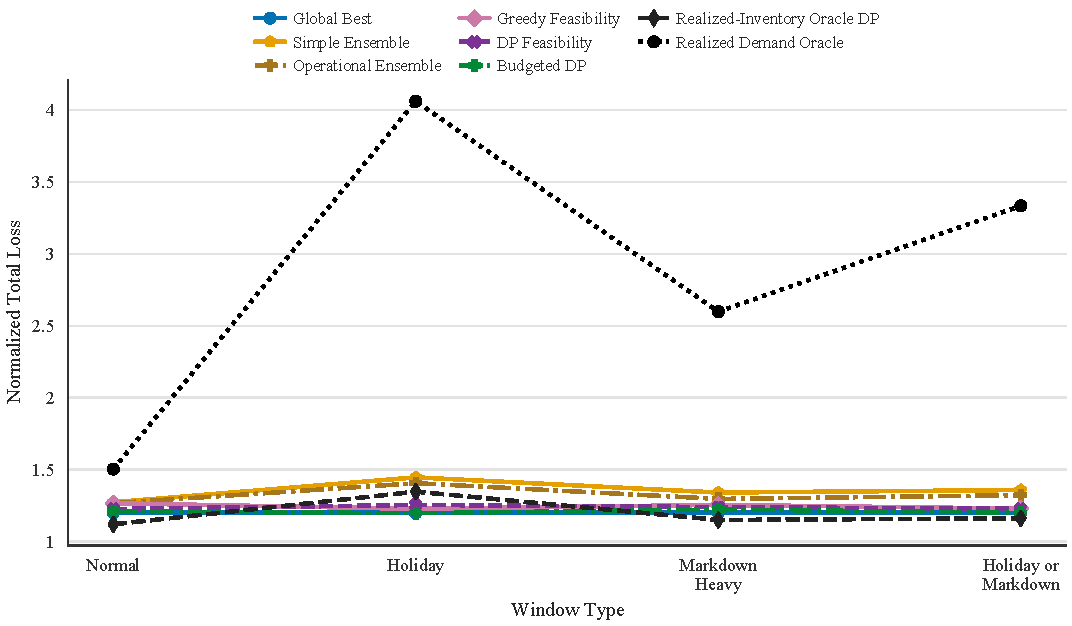
\includegraphics[width=0.85\linewidth]{figures/walmart_window_type_normalized_loss.pdf}
\caption{Walmart normalized planning loss by holiday and markdown stress window.}
\label{fig:walmart-window-normalized-loss}
\end{figure}

\begin{figure}[htbp]
\centering
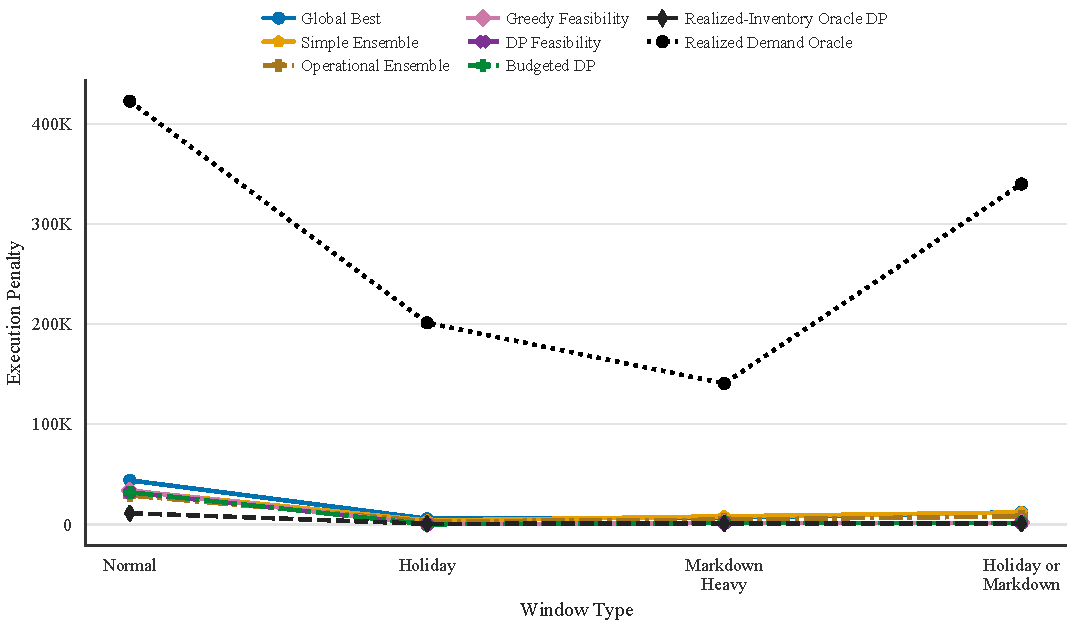
\includegraphics[width=0.85\linewidth]{figures/walmart_window_type_execution_penalty.pdf}
\caption{Walmart execution penalty by holiday and markdown stress window.}
\label{fig:walmart-window-execution-penalty}
\end{figure}

\begin{figure}[htbp]
\centering
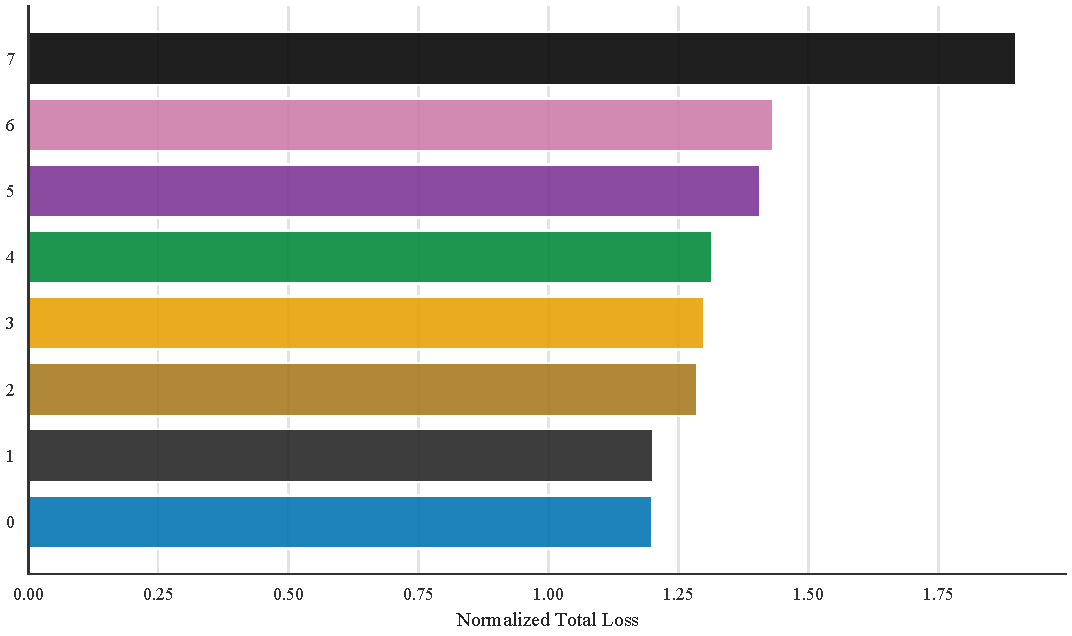
\includegraphics[width=0.85\linewidth]{figures/walmart_weekly_cadence_constraints.pdf}
\caption{Walmart weekly cadence constraint comparison.}
\label{fig:walmart-weekly-cadence}
\end{figure}

\begin{figure}[htbp]
\centering
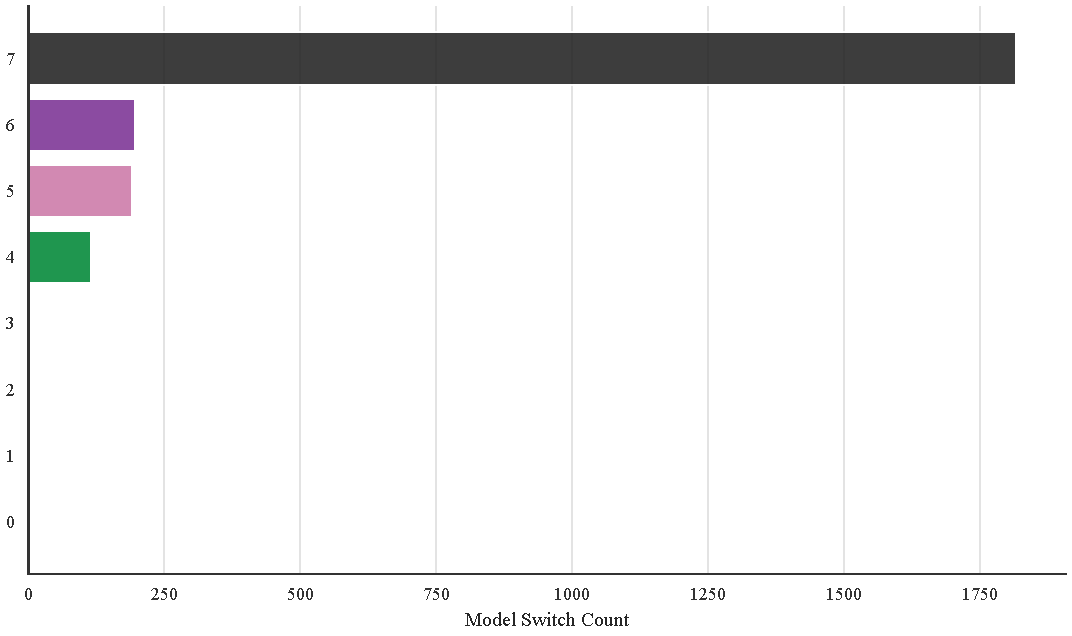
\includegraphics[width=0.85\linewidth]{figures/walmart_budgeted_dp_switching_behavior.pdf}
\caption{Walmart Budgeted-DP switching behavior under weekly cadence constraints.}
\label{fig:walmart-budgeted-dp-switching}
\end{figure}

\section{Citation Completion Notes}

The current draft includes an initial verified reference set for forecasting metrics, retail forecasting benchmarks, inventory control, forecast combination, rolling-horizon decision making, supply-chain planning, and tree-based forecasting models. A later literature pass should still expand coverage of planning nervousness, enterprise planning-system implementation, and execution-risk measurement before submission.


\bibliographystyle{plainnat}
\bibliography{references}

\end{document}
